\documentclass[1p]{elsarticle_modified}
%\bibliographystyle{elsarticle-num}

%\usepackage[colorlinks]{hyperref}
%\usepackage{abbrmath_seonhwa} %\Abb, \Ascr, \Acal ,\Abf, \Afrak
\usepackage{amsfonts}
\usepackage{amssymb}
\usepackage{amsmath}
\usepackage{amsthm}
\usepackage{scalefnt}
\usepackage{amsbsy}
\usepackage{kotex}
\usepackage{caption}
\usepackage{subfig}
\usepackage{color}
\usepackage{graphicx}
\usepackage{xcolor} %% white, black, red, green, blue, cyan, magenta, yellow
\usepackage{float}
\usepackage{setspace}
\usepackage{hyperref}

\usepackage{tikz}
\usetikzlibrary{arrows}

\usepackage{multirow}
\usepackage{array} % fixed length table
\usepackage{hhline}

%%%%%%%%%%%%%%%%%%%%%
\makeatletter
\renewcommand*\env@matrix[1][\arraystretch]{%
	\edef\arraystretch{#1}%
	\hskip -\arraycolsep
	\let\@ifnextchar\new@ifnextchar
	\array{*\c@MaxMatrixCols c}}
\makeatother %https://tex.stackexchange.com/questions/14071/how-can-i-increase-the-line-spacing-in-a-matrix
%%%%%%%%%%%%%%%

\usepackage[normalem]{ulem}

\newcommand{\msout}[1]{\ifmmode\text{\sout{\ensuremath{#1}}}\else\sout{#1}\fi}
%SOURCE: \msout is \stkout macro in https://tex.stackexchange.com/questions/20609/strikeout-in-math-mode

\newcommand{\cancel}[1]{
	\ifmmode
	{\color{red}\msout{#1}}
	\else
	{\color{red}\sout{#1}}
	\fi
}

\newcommand{\add}[1]{
	{\color{blue}\uwave{#1}}
}

\newcommand{\replace}[2]{
	\ifmmode
	{\color{red}\msout{#1}}{\color{blue}\uwave{#2}}
	\else
	{\color{red}\sout{#1}}{\color{blue}\uwave{#2}}
	\fi
}

\newcommand{\Sol}{\mathcal{S}} %segment
\newcommand{\D}{D} %diagram
\newcommand{\A}{\mathcal{A}} %arc


%%%%%%%%%%%%%%%%%%%%%%%%%%%%%5 test

\def\sl{\operatorname{\textup{SL}}(2,\Cbb)}
\def\psl{\operatorname{\textup{PSL}}(2,\Cbb)}
\def\quan{\mkern 1mu \triangleright \mkern 1mu}

\theoremstyle{definition}
\newtheorem{thm}{Theorem}[section]
\newtheorem{prop}[thm]{Proposition}
\newtheorem{lem}[thm]{Lemma}
\newtheorem{ques}[thm]{Question}
\newtheorem{cor}[thm]{Corollary}
\newtheorem{defn}[thm]{Definition}
\newtheorem{exam}[thm]{Example}
\newtheorem{rmk}[thm]{Remark}
\newtheorem{alg}[thm]{Algorithm}

\newcommand{\I}{\sqrt{-1}}
\begin{document}

%\begin{frontmatter}
%
%\title{Boundary parabolic representations of knots up to 8 crossings}
%
%%% Group authors per affiliation:
%\author{Yunhi Cho} 
%\address{Department of Mathematics, University of Seoul, Seoul, Korea}
%\ead{yhcho@uos.ac.kr}
%
%
%\author{Seonhwa Kim} %\fnref{s_kim}}
%\address{Center for Geometry and Physics, Institute for Basic Science, Pohang, 37673, Korea}
%\ead{ryeona17@ibs.re.kr}
%
%\author{Hyuk Kim}
%\address{Department of Mathematical Sciences, Seoul National University, Seoul 08826, Korea}
%\ead{hyukkim@snu.ac.kr}
%
%\author{Seokbeom Yoon}
%\address{Department of Mathematical Sciences, Seoul National University, Seoul, 08826,  Korea}
%\ead{sbyoon15@snu.ac.kr}
%
%\begin{abstract}
%We find all boundary parabolic representation of knots up to 8 crossings.
%
%\end{abstract}
%\begin{keyword}
%    \MSC[2010] 57M25 
%\end{keyword}
%
%\end{frontmatter}

%\linenumbers
%\tableofcontents
%
\newcommand\colored[1]{\textcolor{white}{\rule[-0.35ex]{0.8em}{1.4ex}}\kern-0.8em\color{red} #1}%
%\newcommand\colored[1]{\textcolor{white}{ #1}\kern-2.17ex	\textcolor{white}{ #1}\kern-1.81ex	\textcolor{white}{ #1}\kern-2.15ex\color{red}#1	}

{\Large $\underline{12a_{1105}~(K12a_{1105})}$}

\setlength{\tabcolsep}{10pt}
\renewcommand{\arraystretch}{1.6}
\vspace{1cm}\begin{tabular}{m{100pt}>{\centering\arraybackslash}m{274pt}}
\multirow{5}{120pt}{
	\centering
	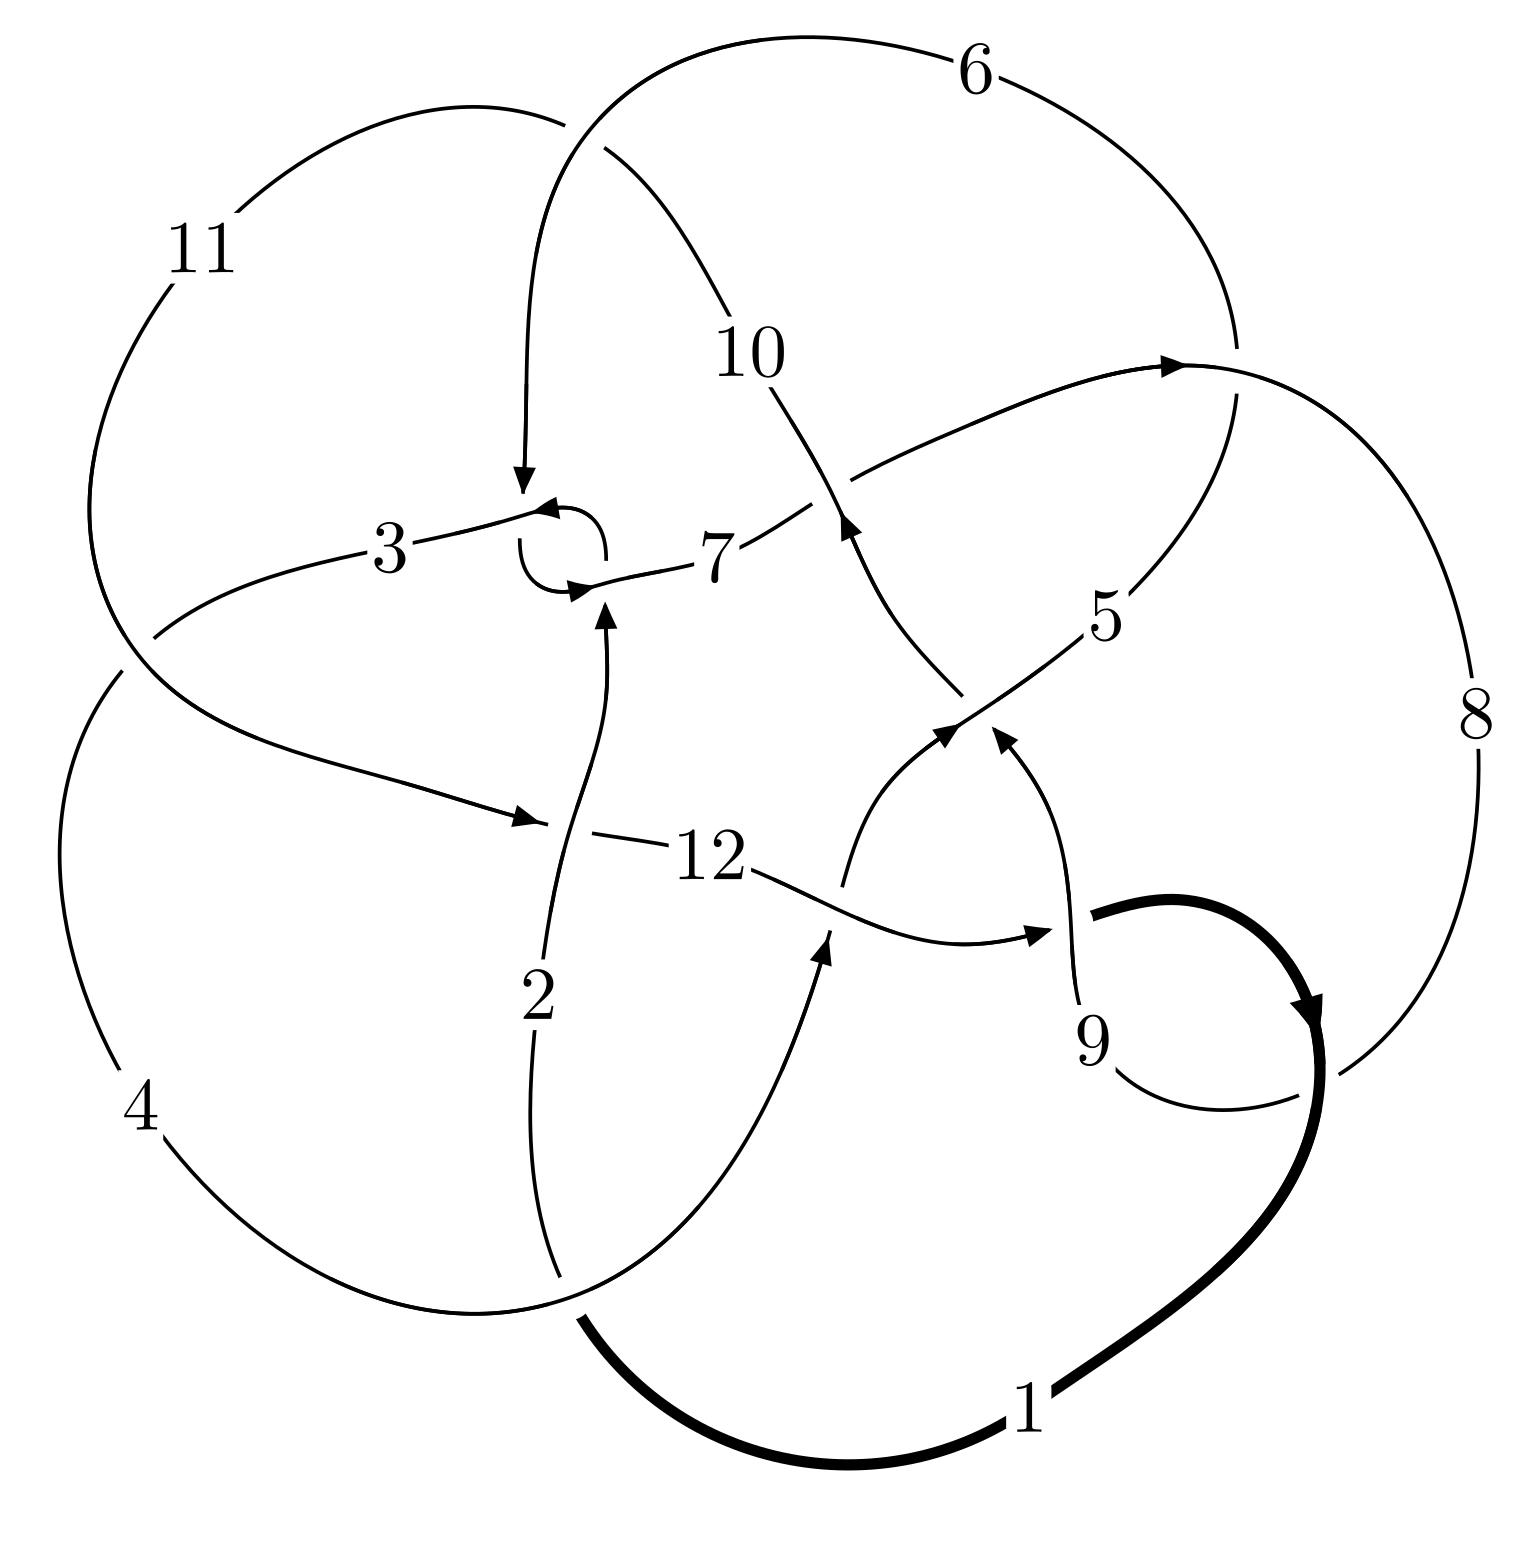
\includegraphics[width=112pt]{../../../GIT/diagram.site/diagram/png/1906_12a_1105.png}\\
\ \ \ A knot diagram\footnotemark}&
\allowdisplaybreaks
\textbf{Linearized knot diagam} \\
\cline{2-2}
 &
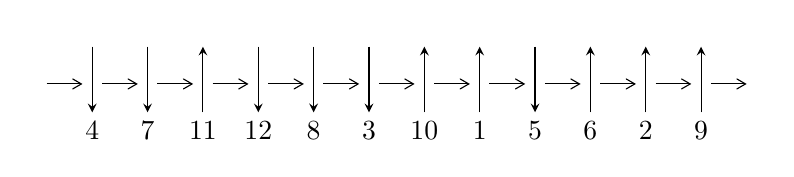
\begin{tikzpicture}[x=20pt, y=17pt]
	% nodes
	\node (C0) at (0, 0) {};
	\node (C1) at (1, 0) {};
	\node (C1U) at (1, +1) {};
	\node (C1D) at (1, -1) {4};

	\node (C2) at (2, 0) {};
	\node (C2U) at (2, +1) {};
	\node (C2D) at (2, -1) {7};

	\node (C3) at (3, 0) {};
	\node (C3U) at (3, +1) {};
	\node (C3D) at (3, -1) {11};

	\node (C4) at (4, 0) {};
	\node (C4U) at (4, +1) {};
	\node (C4D) at (4, -1) {12};

	\node (C5) at (5, 0) {};
	\node (C5U) at (5, +1) {};
	\node (C5D) at (5, -1) {8};

	\node (C6) at (6, 0) {};
	\node (C6U) at (6, +1) {};
	\node (C6D) at (6, -1) {3};

	\node (C7) at (7, 0) {};
	\node (C7U) at (7, +1) {};
	\node (C7D) at (7, -1) {10};

	\node (C8) at (8, 0) {};
	\node (C8U) at (8, +1) {};
	\node (C8D) at (8, -1) {1};

	\node (C9) at (9, 0) {};
	\node (C9U) at (9, +1) {};
	\node (C9D) at (9, -1) {5};

	\node (C10) at (10, 0) {};
	\node (C10U) at (10, +1) {};
	\node (C10D) at (10, -1) {6};

	\node (C11) at (11, 0) {};
	\node (C11U) at (11, +1) {};
	\node (C11D) at (11, -1) {2};

	\node (C12) at (12, 0) {};
	\node (C12U) at (12, +1) {};
	\node (C12D) at (12, -1) {9};
	\node (C13) at (13, 0) {};

	% arrows
	\draw[->,>={angle 60}]
	(C0) edge (C1) (C1) edge (C2) (C2) edge (C3) (C3) edge (C4) (C4) edge (C5) (C5) edge (C6) (C6) edge (C7) (C7) edge (C8) (C8) edge (C9) (C9) edge (C10) (C10) edge (C11) (C11) edge (C12) (C12) edge (C13) ;	\draw[->,>=stealth]
	(C1U) edge (C1D) (C2U) edge (C2D) (C3D) edge (C3U) (C4U) edge (C4D) (C5U) edge (C5D) (C6U) edge (C6D) (C7D) edge (C7U) (C8D) edge (C8U) (C9U) edge (C9D) (C10D) edge (C10U) (C11D) edge (C11U) (C12D) edge (C12U) ;
	\end{tikzpicture} \\
\hhline{~~} \\& 
\textbf{Solving Sequence} \\ \cline{2-2} 
 &
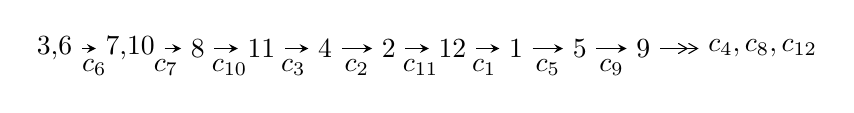
\begin{tikzpicture}[x=23pt, y=7pt]
	% node
	\node (A0) at (-1/8, 0) {3,6};
	\node (A1) at (17/16, 0) {7,10};
	\node (A2) at (17/8, 0) {8};
	\node (A3) at (25/8, 0) {11};
	\node (A4) at (33/8, 0) {4};
	\node (A5) at (41/8, 0) {2};
	\node (A6) at (49/8, 0) {12};
	\node (A7) at (57/8, 0) {1};
	\node (A8) at (65/8, 0) {5};
	\node (A9) at (73/8, 0) {9};
	\node (C1) at (1/2, -1) {$c_{6}$};
	\node (C2) at (13/8, -1) {$c_{7}$};
	\node (C3) at (21/8, -1) {$c_{10}$};
	\node (C4) at (29/8, -1) {$c_{3}$};
	\node (C5) at (37/8, -1) {$c_{2}$};
	\node (C6) at (45/8, -1) {$c_{11}$};
	\node (C7) at (53/8, -1) {$c_{1}$};
	\node (C8) at (61/8, -1) {$c_{5}$};
	\node (C9) at (69/8, -1) {$c_{9}$};
	\node (A10) at (11, 0) {$c_{4},c_{8},c_{12}$};

	% edge
	\draw[->,>=stealth]	
	(A0) edge (A1) (A1) edge (A2) (A2) edge (A3) (A3) edge (A4) (A4) edge (A5) (A5) edge (A6) (A6) edge (A7) (A7) edge (A8) (A8) edge (A9) ;
	\draw[->>,>={angle 60}]	
	(A9) edge (A10);
\end{tikzpicture} \\ 

\end{tabular} \\

\footnotetext{
The image of knot diagram is generated by the software ``\textbf{Draw programme}" developed by Andrew Bartholomew(\url{http://www.layer8.co.uk/maths/draw/index.htm\#Running-draw}), where we modified some parts for our purpose(\url{https://github.com/CATsTAILs/LinksPainter}).
}\phantom \\ \newline 
\centering \textbf{Ideals for irreducible components\footnotemark of $X_{\text{par}}$} 
 
\begin{align*}
I^u_{1}&=\langle 
-1.13930\times10^{21} u^{39}-1.89955\times10^{22} u^{38}+\cdots+1.42950\times10^{21} b+3.75712\times10^{23},\\
\phantom{I^u_{1}}&\phantom{= \langle  }-6.56657\times10^{20} u^{39}-9.62976\times10^{21} u^{38}+\cdots+2.85899\times10^{21} a-1.48932\times10^{23},\\
\phantom{I^u_{1}}&\phantom{= \langle  }u^{40}+17 u^{39}+\cdots-2560 u-256\rangle \\
I^u_{2}&=\langle 
989449936519 u^{27}-4930796017655 u^{26}+\cdots+1798585993788 b-6638482452236,\\
\phantom{I^u_{2}}&\phantom{= \langle  }5649032515717 u^{27}-20633683854770 u^{26}+\cdots+1798585993788 a+15418713106993,\\
\phantom{I^u_{2}}&\phantom{= \langle  }u^{28}-4 u^{27}+\cdots+13 u^2+1\rangle \\
I^u_{3}&=\langle 
-160 u^{59} a-28504115 u^{59}+\cdots+32 a+3787205,\;52235 u^{59} a+20380 u^{59}+\cdots+25702 a+2510,\\
\phantom{I^u_{3}}&\phantom{= \langle  }5 u^{60}-50 u^{59}+\cdots-3 u+1\rangle \\
I^u_{4}&=\langle 
- u^7 a^3+u^7 a^2+\cdots- a+3,\;u^7 a^3- u^7 a^2+\cdots+3 a-1,\\
\phantom{I^u_{4}}&\phantom{= \langle  }u^7 a^2+u^6 a^2- u^7 a+2 u^5 a^2- u^6 a+u^4 a^2- u^5 a+u^3 a^2+u^4 a+u^3 a- u^4+u^2 a+b u+a u+2 u^2+b+2 u+1,\\
\phantom{I^u_{4}}&\phantom{= \langle  }u^8 a^2- u^8 a+\cdots+2 u+1\rangle \\
\\
\end{align*}
\raggedright * 3 irreducible components of $\dim_{\mathbb{C}}=0$, with total 188 representations.\\
\raggedright * 1 irreducible components of $\dim_{\mathbb{C}}=1$ \\
\footnotetext{All coefficients of polynomials are rational numbers. But the coefficients are sometimes approximated in decimal forms when there is not enough margin.}
\newpage
\renewcommand{\arraystretch}{1}
\centering \section*{I. $I^u_{1}= \langle -1.14\times10^{21} u^{39}-1.90\times10^{22} u^{38}+\cdots+1.43\times10^{21} b+3.76\times10^{23},\;-6.57\times10^{20} u^{39}-9.63\times10^{21} u^{38}+\cdots+2.86\times10^{21} a-1.49\times10^{23},\;u^{40}+17 u^{39}+\cdots-2560 u-256 \rangle$}
\flushleft \textbf{(i) Arc colorings}\\
\begin{tabular}{m{7pt} m{180pt} m{7pt} m{180pt} }
\flushright $a_{3}=$&$\begin{pmatrix}0\\u\end{pmatrix}$ \\
\flushright $a_{6}=$&$\begin{pmatrix}1\\0\end{pmatrix}$ \\
\flushright $a_{7}=$&$\begin{pmatrix}1\\u^2\end{pmatrix}$ \\
\flushright $a_{10}=$&$\begin{pmatrix}0.229681 u^{39}+3.36823 u^{38}+\cdots+427.485 u+52.0925\\0.796992 u^{39}+13.2882 u^{38}+\cdots-2417.55 u-262.828\end{pmatrix}$ \\
\flushright $a_{8}=$&$\begin{pmatrix}-0.0129700 u^{39}-0.147174 u^{38}+\cdots-7.46661 u+1.06374\\-0.382727 u^{39}-6.19695 u^{38}+\cdots+911.623 u+101.298\end{pmatrix}$ \\
\flushright $a_{11}=$&$\begin{pmatrix}1.02667 u^{39}+16.6564 u^{38}+\cdots-1990.06 u-210.736\\0.796992 u^{39}+13.2882 u^{38}+\cdots-2417.55 u-262.828\end{pmatrix}$ \\
\flushright $a_{4}=$&$\begin{pmatrix}-0.245169 u^{39}-3.87419 u^{38}+\cdots+753.796 u+88.9443\\-0.293676 u^{39}-4.54829 u^{38}+\cdots+539.688 u+62.7632\end{pmatrix}$ \\
\flushright $a_{2}=$&$\begin{pmatrix}u\\u^3+u\end{pmatrix}$ \\
\flushright $a_{12}=$&$\begin{pmatrix}-0.758262 u^{39}-11.1881 u^{38}+\cdots+54.0332 u+6.22604\\-2.66485 u^{39}-43.7900 u^{38}+\cdots+5568.03 u+593.976\end{pmatrix}$ \\
\flushright $a_{1}=$&$\begin{pmatrix}-0.0107557 u^{39}+0.0107774 u^{38}+\cdots-87.9801 u-3.23265\\-0.503035 u^{39}-8.17030 u^{38}+\cdots+910.250 u+100.732\end{pmatrix}$ \\
\flushright $a_{5}=$&$\begin{pmatrix}-0.0567806 u^{39}-0.898599 u^{38}+\cdots-348.002 u-42.0306\\0.752668 u^{39}+11.5333 u^{38}+\cdots-884.556 u-93.8953\end{pmatrix}$ \\
\flushright $a_{9}=$&$\begin{pmatrix}-1.60236 u^{39}-25.6296 u^{38}+\cdots+1879.61 u+190.846\\-1.79529 u^{39}-29.3126 u^{38}+\cdots+4403.99 u+470.747\end{pmatrix}$\\&\end{tabular}
\flushleft \textbf{(ii) Obstruction class $= -1$}\\~\\
\flushleft \textbf{(iii) Cusp Shapes $= -\frac{100081583463789896653}{47299541498605875888} u^{39}-\frac{168233866403703359237}{5255504610956208432} u^{38}+\cdots+\frac{6734890128933396237742}{2956221343662867243} u+\frac{669015638105036849960}{2956221343662867243}$}\\~\\
\newpage\renewcommand{\arraystretch}{1}
\flushleft \textbf{(iv) u-Polynomials at the component}\newline \\
\begin{tabular}{m{50pt}|m{274pt}}
Crossings & \hspace{64pt}u-Polynomials at each crossing \\
\hline $$\begin{aligned}c_{1},c_{5}\end{aligned}$$&$\begin{aligned}
&u^{40}-3 u^{39}+\cdots-135 u+27
\end{aligned}$\\
\hline $$\begin{aligned}c_{2},c_{6}\end{aligned}$$&$\begin{aligned}
&u^{40}+17 u^{39}+\cdots-2560 u-256
\end{aligned}$\\
\hline $$\begin{aligned}c_{3},c_{10}\end{aligned}$$&$\begin{aligned}
&27(27 u^{40}-27 u^{39}+\cdots+u+1)
\end{aligned}$\\
\hline $$\begin{aligned}c_{4},c_{9}\end{aligned}$$&$\begin{aligned}
&27(27 u^{40}+27 u^{39}+\cdots- u+1)
\end{aligned}$\\
\hline $$\begin{aligned}c_{7},c_{11}\end{aligned}$$&$\begin{aligned}
&u^{40}+3 u^{39}+\cdots+135 u+27
\end{aligned}$\\
\hline $$\begin{aligned}c_{8},c_{12}\end{aligned}$$&$\begin{aligned}
&u^{40}-17 u^{39}+\cdots+2560 u-256
\end{aligned}$\\
\hline
\end{tabular}\\~\\
\newpage\renewcommand{\arraystretch}{1}
\flushleft \textbf{(v) Riley Polynomials at the component}\newline \\
\begin{tabular}{m{50pt}|m{274pt}}
Crossings & \hspace{64pt}Riley Polynomials at each crossing \\
\hline $$\begin{aligned}c_{1},c_{5},c_{7}\\c_{11}\end{aligned}$$&$\begin{aligned}
&y^{40}-7 y^{39}+\cdots+2673 y+729
\end{aligned}$\\
\hline $$\begin{aligned}c_{2},c_{6},c_{8}\\c_{12}\end{aligned}$$&$\begin{aligned}
&y^{40}+17 y^{39}+\cdots+65536 y+65536
\end{aligned}$\\
\hline $$\begin{aligned}c_{3},c_{4},c_{9}\\c_{10}\end{aligned}$$&$\begin{aligned}
&729(729 y^{40}-16767 y^{39}+\cdots-59 y+1)
\end{aligned}$\\
\hline
\end{tabular}\\~\\
\newpage\flushleft \textbf{(vi) Complex Volumes and Cusp Shapes}
$$\begin{array}{c|c|c}  
\text{Solutions to }I^u_{1}& \I (\text{vol} + \sqrt{-1}CS) & \text{Cusp shape}\\
 \hline 
\begin{aligned}
u &= \phantom{-}1.14028\phantom{ +0.000000I} \\
a &= \phantom{-}0.542779\phantom{ +0.000000I} \\
b &= -0.289176\phantom{ +0.000000I}\end{aligned}
 & -0.678004\phantom{ +0.000000I} & -12.8890\phantom{ +0.000000I} \\ \hline\begin{aligned}
u &= -1.139630 + 0.242928 I \\
a &= -0.042870 + 0.308351 I \\
b &= \phantom{-}1.073230 - 0.724091 I\end{aligned}
 & -3.3441 - 15.0894 I & \phantom{-0.000000 } 0 \\ \hline\begin{aligned}
u &= -1.139630 - 0.242928 I \\
a &= -0.042870 - 0.308351 I \\
b &= \phantom{-}1.073230 + 0.724091 I\end{aligned}
 & -3.3441 + 15.0894 I & \phantom{-0.000000 } 0 \\ \hline\begin{aligned}
u &= -0.497516 + 1.077900 I \\
a &= \phantom{-}1.41196 - 0.31741 I \\
b &= -1.15222 - 0.87143 I\end{aligned}
 & \phantom{-}0.79692 + 3.49099 I & \phantom{-0.000000 } 0 \\ \hline\begin{aligned}
u &= -0.497516 - 1.077900 I \\
a &= \phantom{-}1.41196 + 0.31741 I \\
b &= -1.15222 + 0.87143 I\end{aligned}
 & \phantom{-}0.79692 - 3.49099 I & \phantom{-0.000000 } 0 \\ \hline\begin{aligned}
u &= -0.104793 + 1.182780 I \\
a &= \phantom{-}1.52088 - 0.52726 I \\
b &= -1.185540 - 0.504784 I\end{aligned}
 & \phantom{-}3.39633 + 4.91222 I & \phantom{-0.000000 } 0 \\ \hline\begin{aligned}
u &= -0.104793 - 1.182780 I \\
a &= \phantom{-}1.52088 + 0.52726 I \\
b &= -1.185540 + 0.504784 I\end{aligned}
 & \phantom{-}3.39633 - 4.91222 I & \phantom{-0.000000 } 0 \\ \hline\begin{aligned}
u &= -1.180500 + 0.265835 I \\
a &= \phantom{-}0.091123 - 0.306079 I \\
b &= -1.038500 + 0.606550 I\end{aligned}
 & \phantom{-0.000000 } -8.64429 I & \phantom{-0.000000 } 0 \\ \hline\begin{aligned}
u &= -1.180500 - 0.265835 I \\
a &= \phantom{-}0.091123 + 0.306079 I \\
b &= -1.038500 - 0.606550 I\end{aligned}
 & \phantom{-0.000000 -}8.64429 I & \phantom{-0.000000 } 0 \\ \hline\begin{aligned}
u &= \phantom{-}0.069133 + 1.222940 I \\
a &= -1.41555 + 0.34686 I \\
b &= \phantom{-}1.002750 + 0.449758 I\end{aligned}
 & \phantom{-}5.49218 - 1.74539 I & \phantom{-0.000000 } 0\\
 \hline 
 \end{array}$$\newpage$$\begin{array}{c|c|c}  
\text{Solutions to }I^u_{1}& \I (\text{vol} + \sqrt{-1}CS) & \text{Cusp shape}\\
 \hline 
\begin{aligned}
u &= \phantom{-}0.069133 - 1.222940 I \\
a &= -1.41555 - 0.34686 I \\
b &= \phantom{-}1.002750 - 0.449758 I\end{aligned}
 & \phantom{-}5.49218 + 1.74539 I & \phantom{-0.000000 } 0 \\ \hline\begin{aligned}
u &= -0.660444 + 0.377422 I \\
a &= \phantom{-}0.462226 + 0.067787 I \\
b &= \phantom{-}0.245974 - 0.655330 I\end{aligned}
 & -1.29804 + 0.78862 I & -7.24318 - 3.09779 I \\ \hline\begin{aligned}
u &= -0.660444 - 0.377422 I \\
a &= \phantom{-}0.462226 - 0.067787 I \\
b &= \phantom{-}0.245974 + 0.655330 I\end{aligned}
 & -1.29804 - 0.78862 I & -7.24318 + 3.09779 I \\ \hline\begin{aligned}
u &= -1.230810 + 0.195258 I \\
a &= -0.089927 + 0.210729 I \\
b &= \phantom{-}0.767209 - 0.550768 I\end{aligned}
 & -6.55337 - 3.59470 I & \phantom{-0.000000 } 0 \\ \hline\begin{aligned}
u &= -1.230810 - 0.195258 I \\
a &= -0.089927 - 0.210729 I \\
b &= \phantom{-}0.767209 + 0.550768 I\end{aligned}
 & -6.55337 + 3.59470 I & \phantom{-0.000000 } 0 \\ \hline\begin{aligned}
u &= \phantom{-}1.271280 + 0.274737 I \\
a &= -0.327798 + 0.175529 I \\
b &= \phantom{-}0.194769 - 0.082155 I\end{aligned}
 & -5.62477 - 6.34564 I & \phantom{-0.000000 } 0 \\ \hline\begin{aligned}
u &= \phantom{-}1.271280 - 0.274737 I \\
a &= -0.327798 - 0.175529 I \\
b &= \phantom{-}0.194769 + 0.082155 I\end{aligned}
 & -5.62477 + 6.34564 I & \phantom{-0.000000 } 0 \\ \hline\begin{aligned}
u &= -1.31229\phantom{ +0.000000I} \\
a &= \phantom{-}0.170911\phantom{ +0.000000I} \\
b &= -0.718197\phantom{ +0.000000I}\end{aligned}
 & \phantom{-}0.678004\phantom{ +0.000000I} & \phantom{-0.000000 } 0 \\ \hline\begin{aligned}
u &= -1.159260 + 0.636698 I \\
a &= \phantom{-}0.044626 - 0.246409 I \\
b &= -0.425349 + 0.271549 I\end{aligned}
 & -5.49218 + 1.74539 I & \phantom{-0.000000 } 0 \\ \hline\begin{aligned}
u &= -1.159260 - 0.636698 I \\
a &= \phantom{-}0.044626 + 0.246409 I \\
b &= -0.425349 - 0.271549 I\end{aligned}
 & -5.49218 - 1.74539 I & \phantom{-0.000000 } 0\\
 \hline 
 \end{array}$$\newpage$$\begin{array}{c|c|c}  
\text{Solutions to }I^u_{1}& \I (\text{vol} + \sqrt{-1}CS) & \text{Cusp shape}\\
 \hline 
\begin{aligned}
u &= -0.695907 + 1.188770 I \\
a &= -0.880382 + 0.211344 I \\
b &= \phantom{-}0.869437 + 0.526441 I\end{aligned}
 & -3.39633 + 4.91222 I & \phantom{-0.000000 } 0 \\ \hline\begin{aligned}
u &= -0.695907 - 1.188770 I \\
a &= -0.880382 - 0.211344 I \\
b &= \phantom{-}0.869437 - 0.526441 I\end{aligned}
 & -3.39633 - 4.91222 I & \phantom{-0.000000 } 0 \\ \hline\begin{aligned}
u &= -0.16888 + 1.42888 I \\
a &= \phantom{-}0.875872 - 0.142263 I \\
b &= -0.683854 - 0.359026 I\end{aligned}
 & \phantom{-0.000000 -}1.73091 I & \phantom{-0.000000 } 0 \\ \hline\begin{aligned}
u &= -0.16888 - 1.42888 I \\
a &= \phantom{-}0.875872 + 0.142263 I \\
b &= -0.683854 + 0.359026 I\end{aligned}
 & \phantom{-0.000000 } -1.73091 I & \phantom{-0.000000 } 0 \\ \hline\begin{aligned}
u &= -0.63247 + 1.29831 I \\
a &= \phantom{-}1.61971 - 0.26786 I \\
b &= -1.48376 - 0.94120 I\end{aligned}
 & \phantom{-0.000000 -}21.3615 I & \phantom{-0.000000 } 0 \\ \hline\begin{aligned}
u &= -0.63247 - 1.29831 I \\
a &= \phantom{-}1.61971 + 0.26786 I \\
b &= -1.48376 + 0.94120 I\end{aligned}
 & \phantom{-0.000000 } -21.3615 I & \phantom{-0.000000 } 0 \\ \hline\begin{aligned}
u &= -0.64624 + 1.30911 I \\
a &= -1.52479 + 0.29337 I \\
b &= \phantom{-}1.44031 + 0.84855 I\end{aligned}
 & \phantom{-}3.3441 + 15.0894 I & \phantom{-0.000000 } 0 \\ \hline\begin{aligned}
u &= -0.64624 - 1.30911 I \\
a &= -1.52479 - 0.29337 I \\
b &= \phantom{-}1.44031 - 0.84855 I\end{aligned}
 & \phantom{-}3.3441 - 15.0894 I & \phantom{-0.000000 } 0 \\ \hline\begin{aligned}
u &= -0.62417 + 1.33594 I \\
a &= \phantom{-}1.398850 - 0.160563 I \\
b &= -1.23726 - 0.84107 I\end{aligned}
 & -2.88034 + 10.04620 I & \phantom{-0.000000 } 0 \\ \hline\begin{aligned}
u &= -0.62417 - 1.33594 I \\
a &= \phantom{-}1.398850 + 0.160563 I \\
b &= -1.23726 + 0.84107 I\end{aligned}
 & -2.88034 - 10.04620 I & \phantom{-0.000000 } 0\\
 \hline 
 \end{array}$$\newpage$$\begin{array}{c|c|c}  
\text{Solutions to }I^u_{1}& \I (\text{vol} + \sqrt{-1}CS) & \text{Cusp shape}\\
 \hline 
\begin{aligned}
u &= -0.17851 + 1.47621 I \\
a &= -0.946229 + 0.461968 I \\
b &= \phantom{-}0.912818 + 0.160424 I\end{aligned}
 & \phantom{-}6.55337 - 3.59470 I & \phantom{-0.000000 } 0 \\ \hline\begin{aligned}
u &= -0.17851 - 1.47621 I \\
a &= -0.946229 - 0.461968 I \\
b &= \phantom{-}0.912818 - 0.160424 I\end{aligned}
 & \phantom{-}6.55337 + 3.59470 I & \phantom{-0.000000 } 0 \\ \hline\begin{aligned}
u &= -0.21634 + 1.47625 I \\
a &= \phantom{-}0.836758 - 0.579742 I \\
b &= -0.908395 - 0.025097 I\end{aligned}
 & \phantom{-}2.88034 - 10.04620 I & \phantom{-0.000000 } 0 \\ \hline\begin{aligned}
u &= -0.21634 - 1.47625 I \\
a &= \phantom{-}0.836758 + 0.579742 I \\
b &= -0.908395 + 0.025097 I\end{aligned}
 & \phantom{-}2.88034 + 10.04620 I & \phantom{-0.000000 } 0 \\ \hline\begin{aligned}
u &= -0.338539 + 0.326750 I \\
a &= \phantom{-}1.24825 + 1.08328 I \\
b &= \phantom{-}0.919011 - 0.516162 I\end{aligned}
 & -0.79692 + 3.49099 I & \phantom{-}3.06687 - 1.73251 I \\ \hline\begin{aligned}
u &= -0.338539 - 0.326750 I \\
a &= \phantom{-}1.24825 - 1.08328 I \\
b &= \phantom{-}0.919011 + 0.516162 I\end{aligned}
 & -0.79692 - 3.49099 I & \phantom{-}3.06687 + 1.73251 I \\ \hline\begin{aligned}
u &= -0.51178 + 1.44815 I \\
a &= -1.163360 + 0.203861 I \\
b &= \phantom{-}1.046570 + 0.560106 I\end{aligned}
 & \phantom{-}5.62477 + 6.34564 I & \phantom{-0.000000 } 0 \\ \hline\begin{aligned}
u &= -0.51178 - 1.44815 I \\
a &= -1.163360 - 0.203861 I \\
b &= \phantom{-}1.046570 - 0.560106 I\end{aligned}
 & \phantom{-}5.62477 - 6.34564 I & \phantom{-0.000000 } 0 \\ \hline\begin{aligned}
u &= \phantom{-}0.231374 + 0.240170 I \\
a &= \phantom{-}0.27380 - 1.92615 I \\
b &= -0.353506 + 0.377468 I\end{aligned}
 & \phantom{-}1.29804 - 0.78862 I & \phantom{-}7.24318 + 3.09779 I \\ \hline\begin{aligned}
u &= \phantom{-}0.231374 - 0.240170 I \\
a &= \phantom{-}0.27380 + 1.92615 I \\
b &= -0.353506 - 0.377468 I\end{aligned}
 & \phantom{-}1.29804 + 0.78862 I & \phantom{-}7.24318 - 3.09779 I\\
 \hline 
 \end{array}$$\newpage\newpage\renewcommand{\arraystretch}{1}
\centering \section*{II. $I^u_{2}= \langle 9.89\times10^{11} u^{27}-4.93\times10^{12} u^{26}+\cdots+1.80\times10^{12} b-6.64\times10^{12},\;5.65\times10^{12} u^{27}-2.06\times10^{13} u^{26}+\cdots+1.80\times10^{12} a+1.54\times10^{13},\;u^{28}-4 u^{27}+\cdots+13 u^2+1 \rangle$}
\flushleft \textbf{(i) Arc colorings}\\
\begin{tabular}{m{7pt} m{180pt} m{7pt} m{180pt} }
\flushright $a_{3}=$&$\begin{pmatrix}0\\u\end{pmatrix}$ \\
\flushright $a_{6}=$&$\begin{pmatrix}1\\0\end{pmatrix}$ \\
\flushright $a_{7}=$&$\begin{pmatrix}1\\u^2\end{pmatrix}$ \\
\flushright $a_{10}=$&$\begin{pmatrix}-3.14082 u^{27}+11.4722 u^{26}+\cdots-7.75888 u-8.57269\\-0.550127 u^{27}+2.74148 u^{26}+\cdots-4.88174 u+3.69095\end{pmatrix}$ \\
\flushright $a_{8}=$&$\begin{pmatrix}0.791533 u^{27}-3.02387 u^{26}+\cdots-2.73997 u-2.68930\\-0.481655 u^{27}+1.30270 u^{26}+\cdots-3.99918 u-0.309878\end{pmatrix}$ \\
\flushright $a_{11}=$&$\begin{pmatrix}-3.69095 u^{27}+14.2137 u^{26}+\cdots-12.6406 u-4.88174\\-0.550127 u^{27}+2.74148 u^{26}+\cdots-4.88174 u+3.69095\end{pmatrix}$ \\
\flushright $a_{4}=$&$\begin{pmatrix}0.500393 u^{27}-0.727935 u^{26}+\cdots+12.0120 u+4.77242\\1.27364 u^{27}-4.63118 u^{26}+\cdots+5.77242 u-0.500393\end{pmatrix}$ \\
\flushright $a_{2}=$&$\begin{pmatrix}u\\u^3+u\end{pmatrix}$ \\
\flushright $a_{12}=$&$\begin{pmatrix}-4.28175 u^{27}+16.4743 u^{26}+\cdots-15.2405 u-5.85271\\-0.881453 u^{27}+4.04850 u^{26}+\cdots-6.89077 u+2.82253\end{pmatrix}$ \\
\flushright $a_{1}=$&$\begin{pmatrix}0.805857 u^{27}-5.11783 u^{26}+\cdots+1.87723 u-8.50015\\-1.27048 u^{27}+4.47409 u^{26}+\cdots-7.19028 u-1.28751\end{pmatrix}$ \\
\flushright $a_{5}=$&$\begin{pmatrix}-2.62974 u^{27}+10.9428 u^{26}+\cdots-10.3722 u+4.79910\\0.582475 u^{27}-1.68360 u^{26}+\cdots+5.31824 u+1.68675\end{pmatrix}$ \\
\flushright $a_{9}=$&$\begin{pmatrix}4.47203 u^{27}-14.7420 u^{26}+\cdots+8.00604 u+10.7851\\1.97526 u^{27}-9.60197 u^{26}+\cdots+9.33245 u-3.01553\end{pmatrix}$\\&\end{tabular}
\flushleft \textbf{(ii) Obstruction class $= 1$}\\~\\
\flushleft \textbf{(iii) Cusp Shapes $= \frac{3953985943693}{1798585993788} u^{27}-\frac{20451602633597}{1798585993788} u^{26}+\cdots-\frac{24752853561361}{1798585993788} u-\frac{3067689954026}{449646498447}$}\\~\\
\newpage\renewcommand{\arraystretch}{1}
\flushleft \textbf{(iv) u-Polynomials at the component}\newline \\
\begin{tabular}{m{50pt}|m{274pt}}
Crossings & \hspace{64pt}u-Polynomials at each crossing \\
\hline $$\begin{aligned}c_{1},c_{5}\end{aligned}$$&$\begin{aligned}
&u^{28}-3 u^{27}+\cdots-48 u+36
\end{aligned}$\\
\hline $$\begin{aligned}c_{2},c_{12}\end{aligned}$$&$\begin{aligned}
&u^{28}+4 u^{27}+\cdots+13 u^2+1
\end{aligned}$\\
\hline $$\begin{aligned}c_{3},c_{10}\end{aligned}$$&$\begin{aligned}
&4(4 u^{28}+4 u^{27}+\cdots+3 u+1)
\end{aligned}$\\
\hline $$\begin{aligned}c_{4},c_{9}\end{aligned}$$&$\begin{aligned}
&4(4 u^{28}-4 u^{27}+\cdots-3 u+1)
\end{aligned}$\\
\hline $$\begin{aligned}c_{6},c_{8}\end{aligned}$$&$\begin{aligned}
&u^{28}-4 u^{27}+\cdots+13 u^2+1
\end{aligned}$\\
\hline $$\begin{aligned}c_{7},c_{11}\end{aligned}$$&$\begin{aligned}
&u^{28}+3 u^{27}+\cdots+48 u+36
\end{aligned}$\\
\hline
\end{tabular}\\~\\
\newpage\renewcommand{\arraystretch}{1}
\flushleft \textbf{(v) Riley Polynomials at the component}\newline \\
\begin{tabular}{m{50pt}|m{274pt}}
Crossings & \hspace{64pt}Riley Polynomials at each crossing \\
\hline $$\begin{aligned}c_{1},c_{5},c_{7}\\c_{11}\end{aligned}$$&$\begin{aligned}
&y^{28}+7 y^{27}+\cdots+6192 y+1296
\end{aligned}$\\
\hline $$\begin{aligned}c_{2},c_{6},c_{8}\\c_{12}\end{aligned}$$&$\begin{aligned}
&y^{28}+14 y^{27}+\cdots+26 y+1
\end{aligned}$\\
\hline $$\begin{aligned}c_{3},c_{4},c_{9}\\c_{10}\end{aligned}$$&$\begin{aligned}
&16(16 y^{28}-144 y^{27}+\cdots+13 y+1)
\end{aligned}$\\
\hline
\end{tabular}\\~\\
\newpage\flushleft \textbf{(vi) Complex Volumes and Cusp Shapes}
$$\begin{array}{c|c|c}  
\text{Solutions to }I^u_{2}& \I (\text{vol} + \sqrt{-1}CS) & \text{Cusp shape}\\
 \hline 
\begin{aligned}
u &= -0.136648 + 0.946331 I \\
a &= \phantom{-}1.76583 + 0.81451 I \\
b &= -1.200650 + 0.372627 I\end{aligned}
 & \phantom{-0.000000 -}1.17094 I & \phantom{-0.000000 }      -7
0. 10   - 0.0853212 I \\ \hline\begin{aligned}
u &= -0.136648 - 0.946331 I \\
a &= \phantom{-}1.76583 - 0.81451 I \\
b &= -1.200650 - 0.372627 I\end{aligned}
 & \phantom{-0.000000 } -1.17094 I & \phantom{-0.000000 -}     -7
0. 10   + 0.0853212 I \\ \hline\begin{aligned}
u &= \phantom{-}0.177807 + 0.938169 I \\
a &= \phantom{-}1.51071 + 0.88729 I \\
b &= -1.247460 + 0.492279 I\end{aligned}
 & \phantom{-}4.15816 - 3.28640 I & \phantom{-}5.68449 + 2.42731 I \\ \hline\begin{aligned}
u &= \phantom{-}0.177807 - 0.938169 I \\
a &= \phantom{-}1.51071 - 0.88729 I \\
b &= -1.247460 - 0.492279 I\end{aligned}
 & \phantom{-}4.15816 + 3.28640 I & \phantom{-}5.68449 - 2.42731 I \\ \hline\begin{aligned}
u &= \phantom{-}0.873788 + 0.210879 I \\
a &= -0.272534 + 0.199714 I \\
b &= -0.994243 - 0.733917 I\end{aligned}
 & \phantom{-}1.08386 + 4.88595 I & -0.88479 - 6.08182 I \\ \hline\begin{aligned}
u &= \phantom{-}0.873788 - 0.210879 I \\
a &= -0.272534 - 0.199714 I \\
b &= -0.994243 + 0.733917 I\end{aligned}
 & \phantom{-}1.08386 - 4.88595 I & -0.88479 + 6.08182 I \\ \hline\begin{aligned}
u &= -0.634034 + 0.950647 I \\
a &= -0.745266 - 0.027755 I \\
b &= \phantom{-}0.411893 - 0.183179 I\end{aligned}
 & -4.15816 + 3.28640 I & -5.68449 - 2.42731 I \\ \hline\begin{aligned}
u &= -0.634034 - 0.950647 I \\
a &= -0.745266 + 0.027755 I \\
b &= \phantom{-}0.411893 + 0.183179 I\end{aligned}
 & -4.15816 - 3.28640 I & -5.68449 + 2.42731 I \\ \hline\begin{aligned}
u &= -1.028830 + 0.552365 I \\
a &= \phantom{-}0.250126 - 0.345287 I \\
b &= -0.092210 + 0.218091 I\end{aligned}
 & -5.62841 + 2.09236 I & -7.49506 - 8.83052 I \\ \hline\begin{aligned}
u &= -1.028830 - 0.552365 I \\
a &= \phantom{-}0.250126 + 0.345287 I \\
b &= -0.092210 - 0.218091 I\end{aligned}
 & -5.62841 - 2.09236 I & -7.49506 + 8.83052 I\\
 \hline 
 \end{array}$$\newpage$$\begin{array}{c|c|c}  
\text{Solutions to }I^u_{2}& \I (\text{vol} + \sqrt{-1}CS) & \text{Cusp shape}\\
 \hline 
\begin{aligned}
u &= -0.006272 + 1.212530 I \\
a &= -1.33659 - 0.47696 I \\
b &= \phantom{-}1.027810 - 0.369099 I\end{aligned}
 & \phantom{-}5.62841 + 2.09236 I & \phantom{-}7.49506 - 8.83052 I \\ \hline\begin{aligned}
u &= -0.006272 - 1.212530 I \\
a &= -1.33659 + 0.47696 I \\
b &= \phantom{-}1.027810 + 0.369099 I\end{aligned}
 & \phantom{-}5.62841 - 2.09236 I & \phantom{-}7.49506 + 8.83052 I \\ \hline\begin{aligned}
u &= -0.339230 + 0.707931 I \\
a &= \phantom{-}1.52784 - 0.63710 I \\
b &= -0.439616 + 0.736626 I\end{aligned}
 & -5.44803 + 1.13999 I & -6.37606 - 0.43186 I \\ \hline\begin{aligned}
u &= -0.339230 - 0.707931 I \\
a &= \phantom{-}1.52784 + 0.63710 I \\
b &= -0.439616 - 0.736626 I\end{aligned}
 & -5.44803 - 1.13999 I & -6.37606 + 0.43186 I \\ \hline\begin{aligned}
u &= \phantom{-}0.390685 + 1.185710 I \\
a &= -0.840034 - 0.831890 I \\
b &= \phantom{-}1.107050 - 0.013789 I\end{aligned}
 & \phantom{-}5.44803 + 1.13999 I & \phantom{-}6.37606 - 0.43186 I \\ \hline\begin{aligned}
u &= \phantom{-}0.390685 - 1.185710 I \\
a &= -0.840034 + 0.831890 I \\
b &= \phantom{-}1.107050 + 0.013789 I\end{aligned}
 & \phantom{-}5.44803 - 1.13999 I & \phantom{-}6.37606 + 0.43186 I \\ \hline\begin{aligned}
u &= \phantom{-}0.549899 + 1.210700 I \\
a &= -1.71288 - 0.31897 I \\
b &= \phantom{-}1.48225 - 1.01007 I\end{aligned}
 & \phantom{-}4.10977 - 10.09610 I & \phantom{-}1.16490 + 8.56371 I \\ \hline\begin{aligned}
u &= \phantom{-}0.549899 - 1.210700 I \\
a &= -1.71288 + 0.31897 I \\
b &= \phantom{-}1.48225 + 1.01007 I\end{aligned}
 & \phantom{-}4.10977 + 10.09610 I & \phantom{-}1.16490 - 8.56371 I \\ \hline\begin{aligned}
u &= \phantom{-}0.421389 + 1.322980 I \\
a &= \phantom{-}1.42666 - 0.08889 I \\
b &= -0.974358 + 0.969439 I\end{aligned}
 & \phantom{-0.000000 } -12.1531 I & \phantom{-0.000000 -}0. + 9.97979 I \\ \hline\begin{aligned}
u &= \phantom{-}0.421389 - 1.322980 I \\
a &= \phantom{-}1.42666 + 0.08889 I \\
b &= -0.974358 - 0.969439 I\end{aligned}
 & \phantom{-0.000000 -}12.1531 I & \phantom{-0.000000 } 0. - 9.97979 I\\
 \hline 
 \end{array}$$\newpage$$\begin{array}{c|c|c}  
\text{Solutions to }I^u_{2}& \I (\text{vol} + \sqrt{-1}CS) & \text{Cusp shape}\\
 \hline 
\begin{aligned}
u &= \phantom{-}1.401670 + 0.143744 I \\
a &= -0.179789 + 0.033183 I \\
b &= \phantom{-}0.550372 - 0.248416 I\end{aligned}
 & -5.41627 - 6.67339 I & \phantom{-}4.1940 + 14.0424 I \\ \hline\begin{aligned}
u &= \phantom{-}1.401670 - 0.143744 I \\
a &= -0.179789 - 0.033183 I \\
b &= \phantom{-}0.550372 + 0.248416 I\end{aligned}
 & -5.41627 + 6.67339 I & \phantom{-}4.1940 - 14.0424 I \\ \hline\begin{aligned}
u &= -0.012372 + 0.517408 I \\
a &= \phantom{-}2.45831 - 1.35804 I \\
b &= \phantom{-}0.010640 + 1.278440 I\end{aligned}
 & -4.10977 + 10.09610 I & -1.16490 - 8.56371 I \\ \hline\begin{aligned}
u &= -0.012372 - 0.517408 I \\
a &= \phantom{-}2.45831 + 1.35804 I \\
b &= \phantom{-}0.010640 - 1.278440 I\end{aligned}
 & -4.10977 - 10.09610 I & -1.16490 + 8.56371 I \\ \hline\begin{aligned}
u &= \phantom{-}0.47228 + 1.48270 I \\
a &= -1.165310 - 0.144959 I \\
b &= \phantom{-}1.003810 - 0.583498 I\end{aligned}
 & \phantom{-}5.41627 - 6.67339 I & -4.1940 + 14.0424 I \\ \hline\begin{aligned}
u &= \phantom{-}0.47228 - 1.48270 I \\
a &= -1.165310 + 0.144959 I \\
b &= \phantom{-}1.003810 + 0.583498 I\end{aligned}
 & \phantom{-}5.41627 + 6.67339 I & -4.1940 - 14.0424 I \\ \hline\begin{aligned}
u &= -0.130132 + 0.342927 I \\
a &= -2.18708 + 2.27887 I \\
b &= -0.145284 - 0.970139 I\end{aligned}
 & -1.08386 + 4.88595 I & \phantom{-}0.88479 - 6.08182 I \\ \hline\begin{aligned}
u &= -0.130132 - 0.342927 I \\
a &= -2.18708 - 2.27887 I \\
b &= -0.145284 + 0.970139 I\end{aligned}
 & -1.08386 - 4.88595 I & \phantom{-}0.88479 + 6.08182 I\\
 \hline 
 \end{array}$$\newpage\newpage\renewcommand{\arraystretch}{1}
\centering \section*{III. $I^u_{3}= \langle -160 a u^{59}-2.85\times10^{7} u^{59}+\cdots+32 a+3.79\times10^{6},\;52235 u^{59} a+20380 u^{59}+\cdots+25702 a+2510,\;5 u^{60}-50 u^{59}+\cdots-3 u+1 \rangle$}
\flushleft \textbf{(i) Arc colorings}\\
\begin{tabular}{m{7pt} m{180pt} m{7pt} m{180pt} }
\flushright $a_{3}=$&$\begin{pmatrix}0\\u\end{pmatrix}$ \\
\flushright $a_{6}=$&$\begin{pmatrix}1\\0\end{pmatrix}$ \\
\flushright $a_{7}=$&$\begin{pmatrix}1\\u^2\end{pmatrix}$ \\
\flushright $a_{10}=$&$\begin{pmatrix}a\\0.00673854 a u^{59}+1200.48 u^{59}+\cdots-0.00134771 a-159.502\end{pmatrix}$ \\
\flushright $a_{8}=$&$\begin{pmatrix}-657.727 a u^{59}+128.283 u^{59}+\cdots+230.545 a-15.2191\\676.391 a u^{59}+101.012 u^{59}+\cdots+9.54999 a-0.233701\end{pmatrix}$ \\
\flushright $a_{11}=$&$\begin{pmatrix}0.00673854 a u^{59}+1200.48 u^{59}+\cdots+0.998652 a-159.502\\0.00673854 a u^{59}+1200.48 u^{59}+\cdots-0.00134771 a-159.502\end{pmatrix}$ \\
\flushright $a_{4}=$&$\begin{pmatrix}-1200.48 a u^{59}+50.4671 u^{59}+\cdots+159.502 a+72.3128\\101.641 u^{59}-975.234 u^{58}+\cdots+32.5156 u-1.60938\end{pmatrix}$ \\
\flushright $a_{2}=$&$\begin{pmatrix}u\\u^3+u\end{pmatrix}$ \\
\flushright $a_{12}=$&$\begin{pmatrix}\frac{27545}{64} u^{59}-\frac{21845}{4} u^{58}+\cdots+a-\frac{18627}{64}\\-0.00673854 a u^{59}+525.539 u^{59}+\cdots+0.00134771 a-63.3109\end{pmatrix}$ \\
\flushright $a_{1}=$&$\begin{pmatrix}30.5585 a u^{59}+25.4406 u^{59}+\cdots-94.1117 a-64.7600\\-551.703 a u^{59}-131.794 u^{59}+\cdots+60.2781 a+6.54620\end{pmatrix}$ \\
\flushright $a_{5}=$&$\begin{pmatrix}420 u^{59} a+\frac{5445}{32} u^{59}+\cdots+\frac{1049}{8} a+\frac{203}{8}\\-146.867 a u^{59}-181.153 u^{59}+\cdots-51.7203 a-27.6287\end{pmatrix}$ \\
\flushright $a_{9}=$&$\begin{pmatrix}293.697 a u^{59}+509.814 u^{59}+\cdots-55.1769 a+131.475\\-192.985 a u^{59}+861.219 u^{59}+\cdots-28.0905 a-24.3376\end{pmatrix}$\\&\end{tabular}
\flushleft \textbf{(ii) Obstruction class $= -1$}\\~\\
\flushleft \textbf{(iii) Cusp Shapes $= -\frac{1265}{8} u^{59}+\frac{14965}{4} u^{58}+\cdots-\frac{8543}{8} u+\frac{759}{2}$}\\~\\
\newpage\renewcommand{\arraystretch}{1}
\flushleft \textbf{(iv) u-Polynomials at the component}\newline \\
\begin{tabular}{m{50pt}|m{274pt}}
Crossings & \hspace{64pt}u-Polynomials at each crossing \\
\hline $$\begin{aligned}c_{1},c_{5},c_{11}\end{aligned}$$&$\begin{aligned}
&400 u^{120}-5480 u^{119}+\cdots-472919040 u+28339200
\end{aligned}$\\
\hline $$\begin{aligned}c_{2},c_{8},c_{12}\end{aligned}$$&$\begin{aligned}
&(5 u^{60}-50 u^{59}+\cdots-3 u+1)^{2}
\end{aligned}$\\
\hline $$\begin{aligned}c_{3},c_{9}\end{aligned}$$&$\begin{aligned}
&64 u^{120}+192 u^{119}+\cdots+426240000 u+2733137920
\end{aligned}$\\
\hline $$\begin{aligned}c_{4},c_{10}\end{aligned}$$&$\begin{aligned}
&64 u^{120}-192 u^{119}+\cdots-426240000 u+2733137920
\end{aligned}$\\
\hline $$\begin{aligned}c_{6}\end{aligned}$$&$\begin{aligned}
&(5 u^{60}+50 u^{59}+\cdots+3 u+1)^{2}
\end{aligned}$\\
\hline $$\begin{aligned}c_{7}\end{aligned}$$&$\begin{aligned}
&400 u^{120}+5480 u^{119}+\cdots+472919040 u+28339200
\end{aligned}$\\
\hline
\end{tabular}\\~\\
\newpage\renewcommand{\arraystretch}{1}
\flushleft \textbf{(v) Riley Polynomials at the component}\newline \\
\begin{tabular}{m{50pt}|m{274pt}}
Crossings & \hspace{64pt}Riley Polynomials at each crossing \\
\hline $$\begin{aligned}c_{1},c_{5},c_{7}\\c_{11}\end{aligned}$$&$\begin{aligned}
&1.60\times10^{5} y^{120}-7200 y^{119}+\cdots+3.42\times10^{16} y+8.03\times10^{14}
\end{aligned}$\\
\hline $$\begin{aligned}c_{2},c_{6},c_{8}\\c_{12}\end{aligned}$$&$\begin{aligned}
&(25 y^{60}+930 y^{59}+\cdots+15 y+1)^{2}
\end{aligned}$\\
\hline $$\begin{aligned}c_{3},c_{4},c_{9}\\c_{10}\end{aligned}$$&$\begin{aligned}
&4096 y^{120}+1.08\times10^{4} y^{119}+\cdots+2.60\times10^{19} y+7.47\times10^{18}
\end{aligned}$\\
\hline
\end{tabular}\\~\\
\newpage\flushleft \textbf{(vi) Complex Volumes and Cusp Shapes}
$$\begin{array}{c|c|c}  
\text{Solutions to }I^u_{3}& \I (\text{vol} + \sqrt{-1}CS) & \text{Cusp shape}\\
 \hline 
\begin{aligned}
u &= \phantom{-}0.321907 + 0.943564 I \\
a &= -0.211148 + 1.105250 I \\
b &= -0.26256 - 1.99549 I\end{aligned}
 & -3.67203 - 11.90650 I & \phantom{-0.000000 } 0 \\ \hline\begin{aligned}
u &= \phantom{-}0.321907 + 0.943564 I \\
a &= \phantom{-}2.66689 - 0.33653 I \\
b &= -0.687502 + 0.733552 I\end{aligned}
 & -3.67203 - 11.90650 I & \phantom{-0.000000 } 0 \\ \hline\begin{aligned}
u &= \phantom{-}0.321907 - 0.943564 I \\
a &= -0.211148 - 1.105250 I \\
b &= -0.26256 + 1.99549 I\end{aligned}
 & -3.67203 + 11.90650 I & \phantom{-0.000000 } 0 \\ \hline\begin{aligned}
u &= \phantom{-}0.321907 - 0.943564 I \\
a &= \phantom{-}2.66689 + 0.33653 I \\
b &= -0.687502 - 0.733552 I\end{aligned}
 & -3.67203 + 11.90650 I & \phantom{-0.000000 } 0 \\ \hline\begin{aligned}
u &= \phantom{-}0.290898 + 0.962372 I \\
a &= \phantom{-}0.700197 + 0.784048 I \\
b &= -0.75843 - 1.46413 I\end{aligned}
 & -4.84435 - 2.21317 I & \phantom{-0.000000 } 0 \\ \hline\begin{aligned}
u &= \phantom{-}0.290898 + 0.962372 I \\
a &= \phantom{-}2.24984 - 0.55461 I \\
b &= -0.637554 + 0.253876 I\end{aligned}
 & -4.84435 - 2.21317 I & \phantom{-0.000000 } 0 \\ \hline\begin{aligned}
u &= \phantom{-}0.290898 - 0.962372 I \\
a &= \phantom{-}0.700197 - 0.784048 I \\
b &= -0.75843 + 1.46413 I\end{aligned}
 & -4.84435 + 2.21317 I & \phantom{-0.000000 } 0 \\ \hline\begin{aligned}
u &= \phantom{-}0.290898 - 0.962372 I \\
a &= \phantom{-}2.24984 + 0.55461 I \\
b &= -0.637554 - 0.253876 I\end{aligned}
 & -4.84435 + 2.21317 I & \phantom{-0.000000 } 0 \\ \hline\begin{aligned}
u &= -0.204638 + 0.984696 I \\
a &= -1.034140 + 0.554038 I \\
b &= -0.071904 + 0.987935 I\end{aligned}
 & \phantom{-}0.982206 + 0.844454 I & \phantom{-0.000000 } 0 \\ \hline\begin{aligned}
u &= -0.204638 + 0.984696 I \\
a &= -2.26834 - 1.27479 I \\
b &= \phantom{-}1.29204 + 1.40466 I\end{aligned}
 & \phantom{-}0.982206 + 0.844454 I & \phantom{-0.000000 } 0\\
 \hline 
 \end{array}$$\newpage$$\begin{array}{c|c|c}  
\text{Solutions to }I^u_{3}& \I (\text{vol} + \sqrt{-1}CS) & \text{Cusp shape}\\
 \hline 
\begin{aligned}
u &= -0.204638 - 0.984696 I \\
a &= -1.034140 - 0.554038 I \\
b &= -0.071904 - 0.987935 I\end{aligned}
 & \phantom{-}0.982206 - 0.844454 I & \phantom{-0.000000 } 0 \\ \hline\begin{aligned}
u &= -0.204638 - 0.984696 I \\
a &= -2.26834 + 1.27479 I \\
b &= \phantom{-}1.29204 - 1.40466 I\end{aligned}
 & \phantom{-}0.982206 - 0.844454 I & \phantom{-0.000000 } 0 \\ \hline\begin{aligned}
u &= \phantom{-}0.318254 + 0.962466 I \\
a &= \phantom{-}0.026549 - 0.690358 I \\
b &= \phantom{-}0.24232 + 1.66247 I\end{aligned}
 & -0.35565 - 6.64390 I & \phantom{-0.000000 } 0 \\ \hline\begin{aligned}
u &= \phantom{-}0.318254 + 0.962466 I \\
a &= -2.48216 + 0.28024 I \\
b &= \phantom{-}0.850057 - 0.568151 I\end{aligned}
 & -0.35565 - 6.64390 I & \phantom{-0.000000 } 0 \\ \hline\begin{aligned}
u &= \phantom{-}0.318254 - 0.962466 I \\
a &= \phantom{-}0.026549 + 0.690358 I \\
b &= \phantom{-}0.24232 - 1.66247 I\end{aligned}
 & -0.35565 + 6.64390 I & \phantom{-0.000000 } 0 \\ \hline\begin{aligned}
u &= \phantom{-}0.318254 - 0.962466 I \\
a &= -2.48216 - 0.28024 I \\
b &= \phantom{-}0.850057 + 0.568151 I\end{aligned}
 & -0.35565 + 6.64390 I & \phantom{-0.000000 } 0 \\ \hline\begin{aligned}
u &= -0.984855 + 0.363005 I \\
a &= -0.655421 + 0.694738 I \\
b &= \phantom{-}1.049900 - 0.000916 I\end{aligned}
 & -2.65659 + 7.48205 I & \phantom{-0.000000 } 0 \\ \hline\begin{aligned}
u &= -0.984855 + 0.363005 I \\
a &= \phantom{-}0.298474 - 0.194999 I \\
b &= \phantom{-}0.640368 + 0.540116 I\end{aligned}
 & -2.65659 + 7.48205 I & \phantom{-0.000000 } 0 \\ \hline\begin{aligned}
u &= -0.984855 - 0.363005 I \\
a &= -0.655421 - 0.694738 I \\
b &= \phantom{-}1.049900 + 0.000916 I\end{aligned}
 & -2.65659 - 7.48205 I & \phantom{-0.000000 } 0 \\ \hline\begin{aligned}
u &= -0.984855 - 0.363005 I \\
a &= \phantom{-}0.298474 + 0.194999 I \\
b &= \phantom{-}0.640368 - 0.540116 I\end{aligned}
 & -2.65659 - 7.48205 I & \phantom{-0.000000 } 0\\
 \hline 
 \end{array}$$\newpage$$\begin{array}{c|c|c}  
\text{Solutions to }I^u_{3}& \I (\text{vol} + \sqrt{-1}CS) & \text{Cusp shape}\\
 \hline 
\begin{aligned}
u &= -0.304706 + 0.896132 I \\
a &= \phantom{-}0.957243 + 0.856438 I \\
b &= -0.07957 - 1.50726 I\end{aligned}
 & \phantom{-0.000000 -}3.23047 I & \phantom{-0.000000 } 0 \\ \hline\begin{aligned}
u &= -0.304706 + 0.896132 I \\
a &= \phantom{-}1.79637 + 0.39260 I \\
b &= -0.315785 - 0.984822 I\end{aligned}
 & \phantom{-0.000000 -}3.23047 I & \phantom{-0.000000 } 0 \\ \hline\begin{aligned}
u &= -0.304706 - 0.896132 I \\
a &= \phantom{-}0.957243 - 0.856438 I \\
b &= -0.07957 + 1.50726 I\end{aligned}
 & \phantom{-0.000000 } -3.23047 I & \phantom{-0.000000 } 0 \\ \hline\begin{aligned}
u &= -0.304706 - 0.896132 I \\
a &= \phantom{-}1.79637 - 0.39260 I \\
b &= -0.315785 + 0.984822 I\end{aligned}
 & \phantom{-0.000000 } -3.23047 I & \phantom{-0.000000 } 0 \\ \hline\begin{aligned}
u &= -0.159113 + 0.919352 I \\
a &= \phantom{-}0.023781 - 0.297620 I \\
b &= -0.48301 + 1.39389 I\end{aligned}
 & \phantom{-}1.29549 + 0.75677 I & \phantom{-0.000000 } 0 \\ \hline\begin{aligned}
u &= -0.159113 + 0.919352 I \\
a &= -2.49514 - 0.85194 I \\
b &= \phantom{-}0.934786 + 0.596619 I\end{aligned}
 & \phantom{-}1.29549 + 0.75677 I & \phantom{-0.000000 } 0 \\ \hline\begin{aligned}
u &= -0.159113 - 0.919352 I \\
a &= \phantom{-}0.023781 + 0.297620 I \\
b &= -0.48301 - 1.39389 I\end{aligned}
 & \phantom{-}1.29549 - 0.75677 I & \phantom{-0.000000 } 0 \\ \hline\begin{aligned}
u &= -0.159113 - 0.919352 I \\
a &= -2.49514 + 0.85194 I \\
b &= \phantom{-}0.934786 - 0.596619 I\end{aligned}
 & \phantom{-}1.29549 - 0.75677 I & \phantom{-0.000000 } 0 \\ \hline\begin{aligned}
u &= -0.563422 + 0.906939 I \\
a &= \phantom{-}0.369590 - 0.833889 I \\
b &= -0.652128 + 1.007840 I\end{aligned}
 & -4.28468 + 5.58928 I & \phantom{-0.000000 } 0 \\ \hline\begin{aligned}
u &= -0.563422 + 0.906939 I \\
a &= -1.122690 - 0.374955 I \\
b &= -0.001425 + 0.354252 I\end{aligned}
 & -4.28468 + 5.58928 I & \phantom{-0.000000 } 0\\
 \hline 
 \end{array}$$\newpage$$\begin{array}{c|c|c}  
\text{Solutions to }I^u_{3}& \I (\text{vol} + \sqrt{-1}CS) & \text{Cusp shape}\\
 \hline 
\begin{aligned}
u &= -0.563422 - 0.906939 I \\
a &= \phantom{-}0.369590 + 0.833889 I \\
b &= -0.652128 - 1.007840 I\end{aligned}
 & -4.28468 - 5.58928 I & \phantom{-0.000000 } 0 \\ \hline\begin{aligned}
u &= -0.563422 - 0.906939 I \\
a &= -1.122690 + 0.374955 I \\
b &= -0.001425 - 0.354252 I\end{aligned}
 & -4.28468 - 5.58928 I & \phantom{-0.000000 } 0 \\ \hline\begin{aligned}
u &= \phantom{-}0.910138 + 0.143266 I \\
a &= \phantom{-}0.308329 - 0.280726 I \\
b &= \phantom{-}0.947533 + 0.830228 I\end{aligned}
 & \phantom{-}0.35565 + 6.64390 I & \phantom{-0.000000 } 0 \\ \hline\begin{aligned}
u &= \phantom{-}0.910138 + 0.143266 I \\
a &= -0.0917514 - 0.0501821 I \\
b &= -1.064280 - 0.680045 I\end{aligned}
 & \phantom{-}0.35565 + 6.64390 I & \phantom{-0.000000 } 0 \\ \hline\begin{aligned}
u &= \phantom{-}0.910138 - 0.143266 I \\
a &= \phantom{-}0.308329 + 0.280726 I \\
b &= \phantom{-}0.947533 - 0.830228 I\end{aligned}
 & \phantom{-}0.35565 - 6.64390 I & \phantom{-0.000000 } 0 \\ \hline\begin{aligned}
u &= \phantom{-}0.910138 - 0.143266 I \\
a &= -0.0917514 + 0.0501821 I \\
b &= -1.064280 + 0.680045 I\end{aligned}
 & \phantom{-}0.35565 - 6.64390 I & \phantom{-0.000000 } 0 \\ \hline\begin{aligned}
u &= \phantom{-}0.882774 + 0.181268 I \\
a &= -0.129951 + 0.347717 I \\
b &= -1.017010 - 0.715087 I\end{aligned}
 & \phantom{-}1.39107 + 3.59624 I & \phantom{-0.000000 } 0 \\ \hline\begin{aligned}
u &= \phantom{-}0.882774 + 0.181268 I \\
a &= \phantom{-}0.319140 + 0.018071 I \\
b &= \phantom{-}0.945911 + 0.532211 I\end{aligned}
 & \phantom{-}1.39107 + 3.59624 I & \phantom{-0.000000 } 0 \\ \hline\begin{aligned}
u &= \phantom{-}0.882774 - 0.181268 I \\
a &= -0.129951 - 0.347717 I \\
b &= -1.017010 + 0.715087 I\end{aligned}
 & \phantom{-}1.39107 - 3.59624 I & \phantom{-0.000000 } 0 \\ \hline\begin{aligned}
u &= \phantom{-}0.882774 - 0.181268 I \\
a &= \phantom{-}0.319140 - 0.018071 I \\
b &= \phantom{-}0.945911 - 0.532211 I\end{aligned}
 & \phantom{-}1.39107 - 3.59624 I & \phantom{-0.000000 } 0\\
 \hline 
 \end{array}$$\newpage$$\begin{array}{c|c|c}  
\text{Solutions to }I^u_{3}& \I (\text{vol} + \sqrt{-1}CS) & \text{Cusp shape}\\
 \hline 
\begin{aligned}
u &= -0.519961 + 0.729814 I \\
a &= \phantom{-}1.42695 - 0.10017 I \\
b &= -0.444188 - 0.465152 I\end{aligned}
 & -1.56173 + 2.08294 I & \phantom{-0.000000 } 0 \\ \hline\begin{aligned}
u &= -0.519961 + 0.729814 I \\
a &= \phantom{-}0.036719 + 0.306272 I \\
b &= \phantom{-}0.098418 - 1.011180 I\end{aligned}
 & -1.56173 + 2.08294 I & \phantom{-0.000000 } 0 \\ \hline\begin{aligned}
u &= -0.519961 - 0.729814 I \\
a &= \phantom{-}1.42695 + 0.10017 I \\
b &= -0.444188 + 0.465152 I\end{aligned}
 & -1.56173 - 2.08294 I & \phantom{-0.000000 } 0 \\ \hline\begin{aligned}
u &= -0.519961 - 0.729814 I \\
a &= \phantom{-}0.036719 - 0.306272 I \\
b &= \phantom{-}0.098418 + 1.011180 I\end{aligned}
 & -1.56173 - 2.08294 I & \phantom{-0.000000 } 0 \\ \hline\begin{aligned}
u &= \phantom{-}1.095990 + 0.142402 I \\
a &= -0.396890 + 0.128629 I \\
b &= -0.280943 - 0.633355 I\end{aligned}
 & -6.10739 + 5.95943 I & \phantom{-0.000000 } 0 \\ \hline\begin{aligned}
u &= \phantom{-}1.095990 + 0.142402 I \\
a &= -0.345099 - 0.114158 I \\
b &= \phantom{-}0.671021 + 0.649697 I\end{aligned}
 & -6.10739 + 5.95943 I & \phantom{-0.000000 } 0 \\ \hline\begin{aligned}
u &= \phantom{-}1.095990 - 0.142402 I \\
a &= -0.396890 - 0.128629 I \\
b &= -0.280943 + 0.633355 I\end{aligned}
 & -6.10739 - 5.95943 I & \phantom{-0.000000 } 0 \\ \hline\begin{aligned}
u &= \phantom{-}1.095990 - 0.142402 I \\
a &= -0.345099 + 0.114158 I \\
b &= \phantom{-}0.671021 - 0.649697 I\end{aligned}
 & -6.10739 - 5.95943 I & \phantom{-0.000000 } 0 \\ \hline\begin{aligned}
u &= \phantom{-}0.358153 + 1.115160 I \\
a &= \phantom{-}0.843184 + 0.869340 I \\
b &= -0.781423 + 0.661689 I\end{aligned}
 & \phantom{-}4.28468 - 5.58928 I & \phantom{-0.000000 } 0 \\ \hline\begin{aligned}
u &= \phantom{-}0.358153 + 1.115160 I \\
a &= -2.01909 - 0.19074 I \\
b &= \phantom{-}1.68522 - 0.61722 I\end{aligned}
 & \phantom{-}4.28468 - 5.58928 I & \phantom{-0.000000 } 0\\
 \hline 
 \end{array}$$\newpage$$\begin{array}{c|c|c}  
\text{Solutions to }I^u_{3}& \I (\text{vol} + \sqrt{-1}CS) & \text{Cusp shape}\\
 \hline 
\begin{aligned}
u &= \phantom{-}0.358153 - 1.115160 I \\
a &= \phantom{-}0.843184 - 0.869340 I \\
b &= -0.781423 - 0.661689 I\end{aligned}
 & \phantom{-}4.28468 + 5.58928 I & \phantom{-0.000000 } 0 \\ \hline\begin{aligned}
u &= \phantom{-}0.358153 - 1.115160 I \\
a &= -2.01909 + 0.19074 I \\
b &= \phantom{-}1.68522 + 0.61722 I\end{aligned}
 & \phantom{-}4.28468 + 5.58928 I & \phantom{-0.000000 } 0 \\ \hline\begin{aligned}
u &= -0.044759 + 0.769987 I \\
a &= \phantom{-}1.78625 + 1.75828 I \\
b &= -0.98838 - 2.07654 I\end{aligned}
 & -0.982206 - 0.844454 I & \phantom{-0.000000 } 0 \\ \hline\begin{aligned}
u &= -0.044759 + 0.769987 I \\
a &= \phantom{-}2.82275 - 0.80695 I \\
b &= -0.209346 - 0.628594 I\end{aligned}
 & -0.982206 - 0.844454 I & \phantom{-0.000000 } 0 \\ \hline\begin{aligned}
u &= -0.044759 - 0.769987 I \\
a &= \phantom{-}1.78625 - 1.75828 I \\
b &= -0.98838 + 2.07654 I\end{aligned}
 & -0.982206 + 0.844454 I & \phantom{-0.000000 } 0 \\ \hline\begin{aligned}
u &= -0.044759 - 0.769987 I \\
a &= \phantom{-}2.82275 + 0.80695 I \\
b &= -0.209346 + 0.628594 I\end{aligned}
 & -0.982206 + 0.844454 I & \phantom{-0.000000 } 0 \\ \hline\begin{aligned}
u &= \phantom{-}0.330776 + 1.199400 I \\
a &= -0.946469 - 0.989763 I \\
b &= \phantom{-}0.813263 - 0.304525 I\end{aligned}
 & \phantom{-}5.39263 - 1.15812 I & \phantom{-0.000000 } 0 \\ \hline\begin{aligned}
u &= \phantom{-}0.330776 + 1.199400 I \\
a &= \phantom{-}1.57047 + 0.10732 I \\
b &= -1.50830 + 0.58789 I\end{aligned}
 & \phantom{-}5.39263 - 1.15812 I & \phantom{-0.000000 } 0 \\ \hline\begin{aligned}
u &= \phantom{-}0.330776 - 1.199400 I \\
a &= -0.946469 + 0.989763 I \\
b &= \phantom{-}0.813263 + 0.304525 I\end{aligned}
 & \phantom{-}5.39263 + 1.15812 I & \phantom{-0.000000 } 0 \\ \hline\begin{aligned}
u &= \phantom{-}0.330776 - 1.199400 I \\
a &= \phantom{-}1.57047 - 0.10732 I \\
b &= -1.50830 - 0.58789 I\end{aligned}
 & \phantom{-}5.39263 + 1.15812 I & \phantom{-0.000000 } 0\\
 \hline 
 \end{array}$$\newpage$$\begin{array}{c|c|c}  
\text{Solutions to }I^u_{3}& \I (\text{vol} + \sqrt{-1}CS) & \text{Cusp shape}\\
 \hline 
\begin{aligned}
u &= \phantom{-}0.369323 + 0.649111 I \\
a &= \phantom{-}0.243352 + 0.267315 I \\
b &= \phantom{-}0.526307 + 1.292300 I\end{aligned}
 & -4.53004 + 8.84379 I & \phantom{-0.000000 } 0 \\ \hline\begin{aligned}
u &= \phantom{-}0.369323 + 0.649111 I \\
a &= -2.58061 + 0.83239 I \\
b &= \phantom{-}0.728108 - 1.075600 I\end{aligned}
 & -4.53004 + 8.84379 I & \phantom{-0.000000 } 0 \\ \hline\begin{aligned}
u &= \phantom{-}0.369323 - 0.649111 I \\
a &= \phantom{-}0.243352 - 0.267315 I \\
b &= \phantom{-}0.526307 - 1.292300 I\end{aligned}
 & -4.53004 - 8.84379 I & \phantom{-0.000000 } 0 \\ \hline\begin{aligned}
u &= \phantom{-}0.369323 - 0.649111 I \\
a &= -2.58061 - 0.83239 I \\
b &= \phantom{-}0.728108 + 1.075600 I\end{aligned}
 & -4.53004 - 8.84379 I & \phantom{-0.000000 } 0 \\ \hline\begin{aligned}
u &= -0.561022 + 0.471335 I \\
a &= \phantom{-}0.243530 + 0.297277 I \\
b &= \phantom{-}0.243884 + 1.024390 I\end{aligned}
 & -5.39263 - 1.15812 I & \phantom{-0.000000 } 0 \\ \hline\begin{aligned}
u &= -0.561022 + 0.471335 I \\
a &= -1.54085 + 0.77276 I \\
b &= \phantom{-}0.896398 + 0.511751 I\end{aligned}
 & -5.39263 - 1.15812 I & \phantom{-0.000000 } 0 \\ \hline\begin{aligned}
u &= -0.561022 - 0.471335 I \\
a &= \phantom{-}0.243530 - 0.297277 I \\
b &= \phantom{-}0.243884 - 1.024390 I\end{aligned}
 & -5.39263 + 1.15812 I & \phantom{-0.000000 } 0 \\ \hline\begin{aligned}
u &= -0.561022 - 0.471335 I \\
a &= -1.54085 - 0.77276 I \\
b &= \phantom{-}0.896398 - 0.511751 I\end{aligned}
 & -5.39263 + 1.15812 I & \phantom{-0.000000 } 0 \\ \hline\begin{aligned}
u &= \phantom{-}0.374728 + 0.600295 I \\
a &= \phantom{-}0.1176460 - 0.0657947 I \\
b &= -0.587436 - 1.139780 I\end{aligned}
 & -1.39107 + 3.59624 I & \phantom{-0.000000 } 0 \\ \hline\begin{aligned}
u &= \phantom{-}0.374728 + 0.600295 I \\
a &= \phantom{-}2.35353 - 0.58506 I \\
b &= -0.547659 + 0.733776 I\end{aligned}
 & -1.39107 + 3.59624 I & \phantom{-0.000000 } 0\\
 \hline 
 \end{array}$$\newpage$$\begin{array}{c|c|c}  
\text{Solutions to }I^u_{3}& \I (\text{vol} + \sqrt{-1}CS) & \text{Cusp shape}\\
 \hline 
\begin{aligned}
u &= \phantom{-}0.374728 - 0.600295 I \\
a &= \phantom{-}0.1176460 + 0.0657947 I \\
b &= -0.587436 + 1.139780 I\end{aligned}
 & -1.39107 - 3.59624 I & \phantom{-0.000000 } 0 \\ \hline\begin{aligned}
u &= \phantom{-}0.374728 - 0.600295 I \\
a &= \phantom{-}2.35353 + 0.58506 I \\
b &= -0.547659 - 0.733776 I\end{aligned}
 & -1.39107 - 3.59624 I & \phantom{-0.000000 } 0 \\ \hline\begin{aligned}
u &= \phantom{-}0.367071 + 1.260570 I \\
a &= -0.798354 - 0.858019 I \\
b &= \phantom{-}0.931039 - 0.107339 I\end{aligned}
 & \phantom{-}5.87193 - 0.56893 I & \phantom{-0.000000 } 0 \\ \hline\begin{aligned}
u &= \phantom{-}0.367071 + 1.260570 I \\
a &= \phantom{-}1.145840 + 0.516614 I \\
b &= -1.265610 + 0.187097 I\end{aligned}
 & \phantom{-}5.87193 - 0.56893 I & \phantom{-0.000000 } 0 \\ \hline\begin{aligned}
u &= \phantom{-}0.367071 - 1.260570 I \\
a &= -0.798354 + 0.858019 I \\
b &= \phantom{-}0.931039 + 0.107339 I\end{aligned}
 & \phantom{-}5.87193 + 0.56893 I & \phantom{-0.000000 } 0 \\ \hline\begin{aligned}
u &= \phantom{-}0.367071 - 1.260570 I \\
a &= \phantom{-}1.145840 - 0.516614 I \\
b &= -1.265610 - 0.187097 I\end{aligned}
 & \phantom{-}5.87193 + 0.56893 I & \phantom{-0.000000 } 0 \\ \hline\begin{aligned}
u &= \phantom{-}0.295673 + 0.598047 I \\
a &= -0.522578 + 0.581146 I \\
b &= \phantom{-}0.370410 + 1.047480 I\end{aligned}
 & -5.87193 - 0.56893 I & -5.71165 + 2.62808 I \\ \hline\begin{aligned}
u &= \phantom{-}0.295673 + 0.598047 I \\
a &= -2.67253 + 0.19240 I \\
b &= \phantom{-}1.018990 - 0.390536 I\end{aligned}
 & -5.87193 - 0.56893 I & -5.71165 + 2.62808 I \\ \hline\begin{aligned}
u &= \phantom{-}0.295673 - 0.598047 I \\
a &= -0.522578 - 0.581146 I \\
b &= \phantom{-}0.370410 - 1.047480 I\end{aligned}
 & -5.87193 + 0.56893 I & -5.71165 - 2.62808 I \\ \hline\begin{aligned}
u &= \phantom{-}0.295673 - 0.598047 I \\
a &= -2.67253 - 0.19240 I \\
b &= \phantom{-}1.018990 + 0.390536 I\end{aligned}
 & -5.87193 + 0.56893 I & -5.71165 - 2.62808 I\\
 \hline 
 \end{array}$$\newpage$$\begin{array}{c|c|c}  
\text{Solutions to }I^u_{3}& \I (\text{vol} + \sqrt{-1}CS) & \text{Cusp shape}\\
 \hline 
\begin{aligned}
u &= \phantom{-}0.382429 + 1.285840 I \\
a &= \phantom{-}0.513393 + 0.703587 I \\
b &= -0.852984 + 0.063407 I\end{aligned}
 & \phantom{-}4.84435 + 2.21317 I & \phantom{-0.000000 } 0 \\ \hline\begin{aligned}
u &= \phantom{-}0.382429 + 1.285840 I \\
a &= -0.980146 - 0.766268 I \\
b &= \phantom{-}1.116100 + 0.143339 I\end{aligned}
 & \phantom{-}4.84435 + 2.21317 I & \phantom{-0.000000 } 0 \\ \hline\begin{aligned}
u &= \phantom{-}0.382429 - 1.285840 I \\
a &= \phantom{-}0.513393 - 0.703587 I \\
b &= -0.852984 - 0.063407 I\end{aligned}
 & \phantom{-}4.84435 - 2.21317 I & \phantom{-0.000000 } 0 \\ \hline\begin{aligned}
u &= \phantom{-}0.382429 - 1.285840 I \\
a &= -0.980146 + 0.766268 I \\
b &= \phantom{-}1.116100 - 0.143339 I\end{aligned}
 & \phantom{-}4.84435 - 2.21317 I & \phantom{-0.000000 } 0 \\ \hline\begin{aligned}
u &= \phantom{-}0.551013 + 1.224120 I \\
a &= \phantom{-}1.50347 + 0.41968 I \\
b &= -1.36326 + 0.91622 I\end{aligned}
 & \phantom{-}4.53004 - 8.84379 I & \phantom{-0.000000 } 0 \\ \hline\begin{aligned}
u &= \phantom{-}0.551013 + 1.224120 I \\
a &= -1.76358 - 0.29845 I \\
b &= \phantom{-}1.55805 - 0.90773 I\end{aligned}
 & \phantom{-}4.53004 - 8.84379 I & \phantom{-0.000000 } 0 \\ \hline\begin{aligned}
u &= \phantom{-}0.551013 - 1.224120 I \\
a &= \phantom{-}1.50347 - 0.41968 I \\
b &= -1.36326 - 0.91622 I\end{aligned}
 & \phantom{-}4.53004 + 8.84379 I & \phantom{-0.000000 } 0 \\ \hline\begin{aligned}
u &= \phantom{-}0.551013 - 1.224120 I \\
a &= -1.76358 + 0.29845 I \\
b &= \phantom{-}1.55805 + 0.90773 I\end{aligned}
 & \phantom{-}4.53004 + 8.84379 I & \phantom{-0.000000 } 0 \\ \hline\begin{aligned}
u &= \phantom{-}0.542249 + 1.239600 I \\
a &= \phantom{-}1.72699 + 0.12373 I \\
b &= -1.51023 + 1.09918 I\end{aligned}
 & \phantom{-}3.67203 - 11.90650 I & \phantom{-0.000000 } 0 \\ \hline\begin{aligned}
u &= \phantom{-}0.542249 + 1.239600 I \\
a &= -1.69535 - 0.41640 I \\
b &= \phantom{-}1.39839 - 0.93182 I\end{aligned}
 & \phantom{-}3.67203 - 11.90650 I & \phantom{-0.000000 } 0\\
 \hline 
 \end{array}$$\newpage$$\begin{array}{c|c|c}  
\text{Solutions to }I^u_{3}& \I (\text{vol} + \sqrt{-1}CS) & \text{Cusp shape}\\
 \hline 
\begin{aligned}
u &= \phantom{-}0.542249 - 1.239600 I \\
a &= \phantom{-}1.72699 - 0.12373 I \\
b &= -1.51023 - 1.09918 I\end{aligned}
 & \phantom{-}3.67203 + 11.90650 I & \phantom{-0.000000 } 0 \\ \hline\begin{aligned}
u &= \phantom{-}0.542249 - 1.239600 I \\
a &= -1.69535 + 0.41640 I \\
b &= \phantom{-}1.39839 + 0.93182 I\end{aligned}
 & \phantom{-}3.67203 + 11.90650 I & \phantom{-0.000000 } 0 \\ \hline\begin{aligned}
u &= -0.380832 + 1.323190 I \\
a &= \phantom{-}1.19262 - 0.84227 I \\
b &= -0.861585 - 0.399905 I\end{aligned}
 & \phantom{-}2.50586 + 11.87860 I & \phantom{-0.000000 } 0 \\ \hline\begin{aligned}
u &= -0.380832 + 1.323190 I \\
a &= \phantom{-}1.62361 + 0.22942 I \\
b &= -1.51757 - 0.91108 I\end{aligned}
 & \phantom{-}2.50586 + 11.87860 I & \phantom{-0.000000 } 0 \\ \hline\begin{aligned}
u &= -0.380832 - 1.323190 I \\
a &= \phantom{-}1.19262 + 0.84227 I \\
b &= -0.861585 + 0.399905 I\end{aligned}
 & \phantom{-}2.50586 - 11.87860 I & \phantom{-0.000000 } 0 \\ \hline\begin{aligned}
u &= -0.380832 - 1.323190 I \\
a &= \phantom{-}1.62361 - 0.22942 I \\
b &= -1.51757 + 0.91108 I\end{aligned}
 & \phantom{-}2.50586 - 11.87860 I & \phantom{-0.000000 } 0 \\ \hline\begin{aligned}
u &= \phantom{-}0.032535 + 1.376960 I \\
a &= -0.067483 + 1.117620 I \\
b &= \phantom{-}0.16064 - 1.58335 I\end{aligned}
 & \phantom{-0.000000 -}0.520516 I & \phantom{-0.000000 } 0 \\ \hline\begin{aligned}
u &= \phantom{-}0.032535 + 1.376960 I \\
a &= \phantom{-}1.79080 + 0.25687 I \\
b &= -0.644316 - 0.113122 I\end{aligned}
 & \phantom{-0.000000 -}0.520516 I & \phantom{-0.000000 } 0 \\ \hline\begin{aligned}
u &= \phantom{-}0.032535 - 1.376960 I \\
a &= -0.067483 - 1.117620 I \\
b &= \phantom{-}0.16064 + 1.58335 I\end{aligned}
 & \phantom{-0.000000 } -0.520516 I & \phantom{-0.000000 } 0 \\ \hline\begin{aligned}
u &= \phantom{-}0.032535 - 1.376960 I \\
a &= \phantom{-}1.79080 - 0.25687 I \\
b &= -0.644316 + 0.113122 I\end{aligned}
 & \phantom{-0.000000 } -0.520516 I & \phantom{-0.000000 } 0\\
 \hline 
 \end{array}$$\newpage$$\begin{array}{c|c|c}  
\text{Solutions to }I^u_{3}& \I (\text{vol} + \sqrt{-1}CS) & \text{Cusp shape}\\
 \hline 
\begin{aligned}
u &= \phantom{-}0.575559 + 0.132100 I \\
a &= -0.254659 + 1.029720 I \\
b &= -0.899561 - 0.511447 I\end{aligned}
 & \phantom{-}1.56173 + 2.08294 I & \phantom{-}1.60950 - 3.67011 I \\ \hline\begin{aligned}
u &= \phantom{-}0.575559 + 0.132100 I \\
a &= \phantom{-}0.945682 + 0.649198 I \\
b &= \phantom{-}0.732785 - 0.145823 I\end{aligned}
 & \phantom{-}1.56173 + 2.08294 I & \phantom{-}1.60950 - 3.67011 I \\ \hline\begin{aligned}
u &= \phantom{-}0.575559 - 0.132100 I \\
a &= -0.254659 - 1.029720 I \\
b &= -0.899561 + 0.511447 I\end{aligned}
 & \phantom{-}1.56173 - 2.08294 I & \phantom{-}1.60950 + 3.67011 I \\ \hline\begin{aligned}
u &= \phantom{-}0.575559 - 0.132100 I \\
a &= \phantom{-}0.945682 - 0.649198 I \\
b &= \phantom{-}0.732785 + 0.145823 I\end{aligned}
 & \phantom{-}1.56173 - 2.08294 I & \phantom{-}1.60950 + 3.67011 I \\ \hline\begin{aligned}
u &= \phantom{-}0.67143 + 1.25283 I \\
a &= \phantom{-}0.835340 + 0.222425 I \\
b &= -0.990351 + 0.766177 I\end{aligned}
 & \phantom{-}2.65659 - 7.48205 I & \phantom{-0.000000 } 0 \\ \hline\begin{aligned}
u &= \phantom{-}0.67143 + 1.25283 I \\
a &= -1.48861 - 0.39915 I \\
b &= \phantom{-}1.34263 - 0.46958 I\end{aligned}
 & \phantom{-}2.65659 - 7.48205 I & \phantom{-0.000000 } 0 \\ \hline\begin{aligned}
u &= \phantom{-}0.67143 - 1.25283 I \\
a &= \phantom{-}0.835340 - 0.222425 I \\
b &= -0.990351 - 0.766177 I\end{aligned}
 & \phantom{-}2.65659 + 7.48205 I & \phantom{-0.000000 } 0 \\ \hline\begin{aligned}
u &= \phantom{-}0.67143 - 1.25283 I \\
a &= -1.48861 + 0.39915 I \\
b &= \phantom{-}1.34263 + 0.46958 I\end{aligned}
 & \phantom{-}2.65659 + 7.48205 I & \phantom{-0.000000 } 0 \\ \hline\begin{aligned}
u &= \phantom{-}0.58417 + 1.29672 I \\
a &= -1.071870 + 0.156151 I \\
b &= \phantom{-}0.94658 - 1.11184 I\end{aligned}
 & -2.50586 - 11.87860 I & \phantom{-0.000000 } 0 \\ \hline\begin{aligned}
u &= \phantom{-}0.58417 + 1.29672 I \\
a &= \phantom{-}1.60547 + 0.20718 I \\
b &= -1.166070 + 0.720746 I\end{aligned}
 & -2.50586 - 11.87860 I & \phantom{-0.000000 } 0\\
 \hline 
 \end{array}$$\newpage$$\begin{array}{c|c|c}  
\text{Solutions to }I^u_{3}& \I (\text{vol} + \sqrt{-1}CS) & \text{Cusp shape}\\
 \hline 
\begin{aligned}
u &= \phantom{-}0.58417 - 1.29672 I \\
a &= -1.071870 - 0.156151 I \\
b &= \phantom{-}0.94658 + 1.11184 I\end{aligned}
 & -2.50586 + 11.87860 I & \phantom{-0.000000 } 0 \\ \hline\begin{aligned}
u &= \phantom{-}0.58417 - 1.29672 I \\
a &= \phantom{-}1.60547 - 0.20718 I \\
b &= -1.166070 - 0.720746 I\end{aligned}
 & -2.50586 + 11.87860 I & \phantom{-0.000000 } 0 \\ \hline\begin{aligned}
u &= -0.40259 + 1.37690 I \\
a &= -1.059920 + 0.600086 I \\
b &= \phantom{-}0.839133 + 0.405350 I\end{aligned}
 & \phantom{-}6.10739 + 5.95943 I & \phantom{-0.000000 } 0 \\ \hline\begin{aligned}
u &= -0.40259 + 1.37690 I \\
a &= -1.402550 - 0.068041 I \\
b &= \phantom{-}1.29550 + 0.70878 I\end{aligned}
 & \phantom{-}6.10739 + 5.95943 I & \phantom{-0.000000 } 0 \\ \hline\begin{aligned}
u &= -0.40259 - 1.37690 I \\
a &= -1.059920 - 0.600086 I \\
b &= \phantom{-}0.839133 - 0.405350 I\end{aligned}
 & \phantom{-}6.10739 - 5.95943 I & \phantom{-0.000000 } 0 \\ \hline\begin{aligned}
u &= -0.40259 - 1.37690 I \\
a &= -1.402550 + 0.068041 I \\
b &= \phantom{-}1.29550 - 0.70878 I\end{aligned}
 & \phantom{-}6.10739 - 5.95943 I & \phantom{-0.000000 } 0 \\ \hline\begin{aligned}
u &= -0.129167 + 0.122817 I \\
a &= \phantom{-}0.78075 - 5.53107 I \\
b &= \phantom{-}0.336444 - 1.032790 I\end{aligned}
 & -1.29549 - 0.75677 I & -5.76024 + 1.81125 I \\ \hline\begin{aligned}
u &= -0.129167 + 0.122817 I \\
a &= \phantom{-}6.02259 - 1.91348 I \\
b &= -0.661849 - 0.985048 I\end{aligned}
 & -1.29549 - 0.75677 I & -5.76024 + 1.81125 I \\ \hline\begin{aligned}
u &= -0.129167 - 0.122817 I \\
a &= \phantom{-}0.78075 + 5.53107 I \\
b &= \phantom{-}0.336444 + 1.032790 I\end{aligned}
 & -1.29549 + 0.75677 I & -5.76024 - 1.81125 I \\ \hline\begin{aligned}
u &= -0.129167 - 0.122817 I \\
a &= \phantom{-}6.02259 + 1.91348 I \\
b &= -0.661849 + 0.985048 I\end{aligned}
 & -1.29549 + 0.75677 I & -5.76024 - 1.81125 I\\
 \hline 
 \end{array}$$\newpage\newpage\renewcommand{\arraystretch}{1}
\centering \section*{IV. $I^u_{4}= \langle - u^7 a^3+u^7 a^2+\cdots- a+3,\;u^7 a^3- u^7 a^2+\cdots+3 a-1,\;u^7 a^2- u^7 a+\cdots+b+1,\;u^8 a^2- u^8 a+\cdots+2 u+1 \rangle$}
\flushleft \textbf{(i) Arc colorings}\\
\begin{tabular}{m{7pt} m{180pt} m{7pt} m{180pt} }
\flushright $a_{3}=$&$\begin{pmatrix}0\\u\end{pmatrix}$ \\
\flushright $a_{6}=$&$\begin{pmatrix}1\\0\end{pmatrix}$ \\
\flushright $a_{7}=$&$\begin{pmatrix}1\\u^2\end{pmatrix}$ \\
\flushright $a_{10}=$&$\begin{pmatrix}a\\b\end{pmatrix}$ \\
\flushright $a_{8}=$&$\begin{pmatrix}\frac{1}{2} u^7 a^3-\frac{1}{2} u^7 a^2+\cdots+\frac{3}{2} a+\frac{1}{2}\\u^6 a^2- u^6 a+\cdots+b+2\end{pmatrix}$ \\
\flushright $a_{11}=$&$\begin{pmatrix}b+a\\b\end{pmatrix}$ \\
\flushright $a_{4}=$&$\begin{pmatrix}-\frac{1}{2} u^7 a^3+\frac{1}{2} u^7 a^2+\cdots+\frac{1}{2} a-\frac{1}{2}\\- u^6 a^2+u^6 a-2 u^4 a^2+u^4 a- a^2 u^2- u^3 a+u^3- a u- u^2\end{pmatrix}$ \\
\flushright $a_{2}=$&$\begin{pmatrix}u\\u^3+u\end{pmatrix}$ \\
\flushright $a_{12}=$&$\begin{pmatrix}- u^3 a+u^3- a u+a-1\\- u^7 a^2+u^7 a+\cdots- b-3\end{pmatrix}$ \\
\flushright $a_{1}=$&$\begin{pmatrix}-\frac{1}{2} u^7 a^4+\frac{1}{4} u^7 a^3+\cdots-\frac{1}{4} a-\frac{7}{4}\\- u^7 a^2+u^7 a+\cdots- b-3\end{pmatrix}$ \\
\flushright $a_{5}=$&$\begin{pmatrix}- u^7 a^3+u^7 a^2+\cdots- a-1\\\frac{1}{2} u^7 a^3-\frac{3}{2} u^7 a^2+\cdots+\frac{1}{2} a-\frac{5}{2}\end{pmatrix}$ \\
\flushright $a_{9}=$&$\begin{pmatrix}-\frac{1}{2} u^7 a^4+\frac{7}{4} u^7 a^3+\cdots+\frac{5}{4} a+\frac{3}{4}\\u^4 a- u^4+u^2 a- a u+u\end{pmatrix}$\\&\end{tabular}
\flushleft \textbf{(ii) Obstruction class $= 1$}\\~\\
\flushleft \textbf{(iii) Cusp Shapes $= 0$}\\~\\
\flushleft \textbf{(iv) u-Polynomials at the component} : It cannot be defined for a positive dimension component.\\~\\
\flushleft \textbf{(v) Riley Polynomials at the component} : It cannot be defined for a positive dimension component.\\~\\
\newpage\flushleft \textbf{(iv) Complex Volumes and Cusp Shapes}
$$\begin{array}{c|c|c} 
\text{Solution to }I^u_{4}& \I (\text{vol} + \sqrt{-1}CS) & \text{Cusp shape}\\
 \hline 
\begin{aligned}
u &= \cdots \\
a &= \cdots \\
b &= \cdots\end{aligned}
 & \phantom{-0.000000 } 0 & \phantom{-0.000000 } 0\\
 \hline 
 \end{array}
$$
\newpage\renewcommand{\arraystretch}{1}
\centering \section*{ V. u-Polynomials}
\begin{tabular}{m{50pt}|m{274pt}}
Crossings & \hspace{64pt}u-Polynomials at each crossing \\
\hline $$\begin{aligned}c_{1},c_{5}\end{aligned}$$&$\begin{aligned}
&(u^{28}-3 u^{27}+\cdots-48 u+36)(u^{40}-3 u^{39}+\cdots-135 u+27)
\end{aligned}$\\
\hline $$\begin{aligned}c_{2}\end{aligned}$$&$\begin{aligned}
&(u^{28}+4 u^{27}+\cdots+13 u^2+1)(u^{40}+17 u^{39}+\cdots-2560 u-256)
\end{aligned}$\\
\hline $$\begin{aligned}c_{3},c_{10}\end{aligned}$$&$\begin{aligned}
&108(4 u^{28}+4 u^{27}+\cdots+3 u+1)(27 u^{40}-27 u^{39}+\cdots+u+1)
\end{aligned}$\\
\hline $$\begin{aligned}c_{4},c_{9}\end{aligned}$$&$\begin{aligned}
&108(4 u^{28}-4 u^{27}+\cdots-3 u+1)(27 u^{40}+27 u^{39}+\cdots- u+1)
\end{aligned}$\\
\hline $$\begin{aligned}c_{6}\end{aligned}$$&$\begin{aligned}
&(u^{28}-4 u^{27}+\cdots+13 u^2+1)(u^{40}+17 u^{39}+\cdots-2560 u-256)
\end{aligned}$\\
\hline $$\begin{aligned}c_{7},c_{11}\end{aligned}$$&$\begin{aligned}
&(u^{28}+3 u^{27}+\cdots+48 u+36)(u^{40}+3 u^{39}+\cdots+135 u+27)
\end{aligned}$\\
\hline $$\begin{aligned}c_{8}\end{aligned}$$&$\begin{aligned}
&(u^{28}-4 u^{27}+\cdots+13 u^2+1)(u^{40}-17 u^{39}+\cdots+2560 u-256)
\end{aligned}$\\
\hline $$\begin{aligned}c_{12}\end{aligned}$$&$\begin{aligned}
&(u^{28}+4 u^{27}+\cdots+13 u^2+1)(u^{40}-17 u^{39}+\cdots+2560 u-256)
\end{aligned}$\\
\hline
\end{tabular}\newpage\renewcommand{\arraystretch}{1}
\centering \section*{ VI. Riley Polynomials}
\begin{tabular}{m{50pt}|m{274pt}}
Crossings & \hspace{64pt}Riley Polynomials at each crossing \\
\hline $$\begin{aligned}c_{1},c_{5},c_{7}\\c_{11}\end{aligned}$$&$\begin{aligned}
&(y^{28}+7 y^{27}+\cdots+6192 y+1296)(y^{40}-7 y^{39}+\cdots+2673 y+729)
\end{aligned}$\\
\hline $$\begin{aligned}c_{2},c_{6},c_{8}\\c_{12}\end{aligned}$$&$\begin{aligned}
&(y^{28}+14 y^{27}+\cdots+26 y+1)(y^{40}+17 y^{39}+\cdots+65536 y+65536)
\end{aligned}$\\
\hline $$\begin{aligned}c_{3},c_{4},c_{9}\\c_{10}\end{aligned}$$&$\begin{aligned}
&11664(16 y^{28}-144 y^{27}+\cdots+13 y+1)\\
&\cdot(729 y^{40}-16767 y^{39}+\cdots-59 y+1)
\end{aligned}$\\
\hline
\end{tabular}
\vskip 2pc
\end{document}